\section{Considerações Iniciais}

Conforme discutido anteriormente, a acessibilidade em ambientes de aprendizagem é uma necessidade crescente na era digital, onde as TICs desempenham um papel crucial ao tornar os conteúdos educacionais acessíveis a todos os alunos, independentemente de suas individualidades físicas ou sensoriais \cite{Mayer2021}. Neste contexto, o presente trabalho de doutorado investiga como o enriquecimento de OAs com transcrições e legendas automáticas pode aumentar a inclusão e o engajamento na educação \cite{FalvoJr2023_HICSS, FalvoJr2024_FIE}.

O conceito de OAs é central para as práticas pedagógicas atuais, pois esses recursos digitais flexíveis podem ser reutilizados para apoiar o processo de ensino-aprendizagem \cite{Parakh2022}. A principal contribuição deste trabalho de doutorado é a arquitetura \textit{Speech2Learning}, que propõe o aprimoramento de OAs audíveis por meio de tecnologias de ASR/STT, promovendo a geração automática de legendas, transcrições ou traduções. Dessa forma, videoaulas podem se tornar acessíveis em diferentes línguas e até mesmo sinalizadas por avatares de línguas de sinais baseados em texto.

Este capítulo detalha a aplicação prática da \textit{Speech2Learning} por meio de dois estudos de caso, concebidos como instâncias concretas da arquitetura. Cada estudo (\autoref{c4:cs1} e \autoref{c4:cs2}) segue uma estrutura comum, com subseções que abordam: a implementação e integração da arquitetura \textit{Speech2Learning}; a solução desenvolvida como prova de conceito; os métodos utilizados; e os resultados, com discussões sobre as implicações para a acessibilidade educacional e a arquitetura.

Esses estudos foram conduzidos em colaboração com a \textit{EdTech} brasileira DIO, que desempenhou um papel essencial ao viabilizar avaliações empíricas em OAs de uma plataforma educacional real, marcando um passo significativo na direção de soluções mais acessíveis e inclusivas. Todos os procedimentos éticos relacionados aos estudos de caso foram aprovados pelo CEP, conforme CAAE 78381524.3.0000.5390, em conformidade com as diretrizes exigidas.

\section{Estudo de Caso 1: Legendas em Videoaulas}
\label{c4:cs1}

O primeiro estudo de caso buscou investigar a precisão dos principais serviços de ASR, uma vez que essa tecnologia é central na arquitetura \textit{Speech2Learning}. Na prática, foi utilizado um conjunto de recursos educacionais, disponíveis na plataforma de \textit{e-learning} da DIO, para a construção de uma \sigla{POC}{Prova de Conceito} focada na transcrição e legendagem desses OAs através de serviços de ASR.

Sendo assim, o objetivo do estudo foi expandir a compreensão sobre o papel das transcrições automáticas no processo de ensino-aprendizagem mais acessível. Para isso, foi discutida a convergência dos resultados quantitativos e qualitativos obtidos a partir de três fontes de evidência, seguindo a premissa da metodologia de triangulação de dados \cite{LimaJunior2021}.

Segundo \cite{Farquhar2020}, é possível explorar múltiplas fontes de evidências (quantitativas e/ou qualitativas) e discutir suas respectivas convergências por meio de uma abordagem de triangulação de dados. No contexto deste estudo de caso, as seguintes fontes foram observadas: 
\begin{enumerate}[label=(\roman*)]
    \item Métodos de similaridade léxica;
    \item Respostas de um \textit{survey} anônimo;
    \item Estudos de uma pesquisa documental complementar.
\end{enumerate}

As subseções a seguir exploram o estudo em detalhes, abordando desde a relação com a arquitetura \textit{Speech2Learning} e a implementação de uma POC em colaboração com a \textit{EdTech} DIO, até os pormenores metodológicos e os resultados alcançados.

\subsection{Relação com a Arquitetura \textit{Speech2Learning}}

No primeiro estudo de caso, a arquitetura \textit{Speech2Learning} foi implementada como uma API REST, projetada para seguir rigorosamente as responsabilidades de suas camadas e os padrões do estilo arquitetural REST. A adoção da \textit{Speech2Learning} forneceu diretrizes claras para a separação de interesses entre as camadas da API, facilitando a manutenção e a testabilidade do sistema, além de permitir a substituição ágil do serviço de ASR. Esse \textit{design} modular garante que diferentes provedores de ASR possam ser integrados ou trocados sem grandes impactos na estrutura da API, preservando a consistência e a transparência no funcionamento geral.

Outro diferencial da \textit{Speech2Learning} está na sua aderência a padrões de metadados dos OAs, assegurando que esses recursos sejam enriquecidos com transcrições e legendas de forma padronizada. Essa característica facilita a reutilização dos OAs em diversos contextos educacionais, garantindo acessibilidade e consistência em termos de estrutura e conteúdo.

Embora a avaliação do estudo de caso se concentre na instância concreta da arquitetura, a flexibilidade inerente à \textit{Speech2Learning} possibilitou a criação de uma API robusta, capaz de se conectar a múltiplos serviços de ASR. Esses serviços são implementados por meio de \textit{Gateways} que seguem uma interface comum, permitindo a troca entre componentes de forma transparente e eficiente. Essa abordagem permite uma avaliação abrangente dos provedores de ASR, sem comprometer a integridade da API ou dos OAs gerados.

Simplificando, a relação entre a \textit{Speech2Learning} e este estudo de caso resultou em uma API REST construída em conformidade com os \textit{guidelines} da arquitetura. Na prática, a \textit{Speech2Learning} atende a um requisito essencial deste estudo, que é a necessidade de múltiplos provedores de ASR/STT desacoplados para a geração e avaliação das transcrições automáticas de videoaulas. Para isso, foi iniciada uma POC estratégica com o objetivo de mensurar a complexidade do desenvolvimento e a viabilidade técnica (inicialmente com um único provedor).

A POC é detalhada a seguir e representa a primeira instância concreta da \textit{Speech2Learning}. Sendo assim, essa implementação proporcionou inúmeros aprendizados e explorou a essência da arquitetura, promovendo a acessibilidade por meio do ASR em OAs existentes na plataforma educacional da DIO. A oportunidade de testar a arquitetura em um ecossistema de aprendizagem real foi um passo significativo para a maturidade da \textit{Speech2Learning}.

\subsection{Prova de Conceito: API REST para Legendar Videoaulas}

O desenvolvimento de uma POC, primeira instância da \textit{Speech2Learning}, surgiu de uma necessidade de negócio da \textit{EdTech} DIO de legendar suas videoaulas de forma escalável. Para isso, uma API REST foi implementada para transcrever videoaulas curtas (entre 15 e 30 segundos), algo comum considerando o conceito de \textit{microlearning} adaptado pela DIO para suas necessidades educacionais. 

Com isso, foi possível explorar os padrões de metadados inerentes à arquitetura \textit{Speech2Learning} e gerar transcrições e legendas para videoaulas em múltiplos idiomas. Nesse sentido, foi definido o escopo da POC aos idiomas suportados na plataforma da DIO (Português, Inglês e Espanhol), sendo possível ampliar a acessibilidade desses OAs por meio de transcrições e legendas geradas automaticamente a priori.

Conforme ilustrado no diagrama da \autoref{fig:chapter4-cs1-poc-diagram}, a API segue as diretrizes da arquitetura, apresentando uma estrutura coerente de componentes e conectores, conforme descrito em \citeonline{Bass2021}. O esquema de cores reflete as camadas da \textit{Speech2Learning}, destacando uma implementação que respeita os limites lógicos e as recomendações semânticas estabelecidas. Nesse contexto, a correspondência torna-se ainda mais evidente ao observar os pacotes que organizam os componentes: Infraestrutura (azul), Adaptadores (verde), Casos de Uso (vermelho) e LOs (amarelo).

\begin{figure}[htb]
\centering
\caption{Visão 1ª Instância da \textit{Speech2Learning}: API REST para Legendar Videoaulas}
\label{fig:chapter4-cs1-poc-diagram}
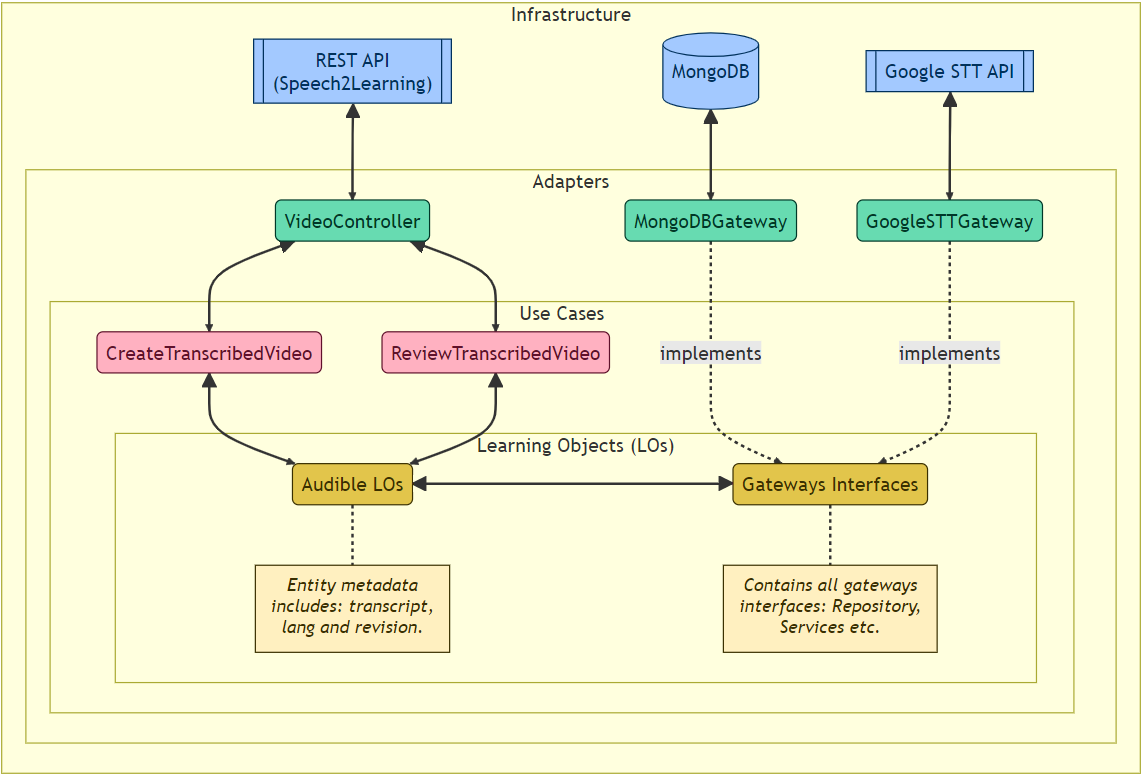
\includegraphics[width=\columnwidth]{images/chapter4-cs1-poc-diagram.png}
\fdireta{FalvoJr2023_HICSS}
\end{figure}

O diagrama define dois \textit{Casos de Uso} relacionados à transcrição de vídeos: \textit{Criar} e \textit{Revisar}. Esta visão é interessante pois esclarece as funcionalidades implementadas na POC. Além disso, as entidades foram projetadas como \textit{OAs Audíveis}, uma vez que são consideradas videoaulas. Para concluir, detalhes sobre a implementação também são expostos claramente na camada de \textit{Infraestrutura}. Por exemplo, o ponto de entrada é uma \textit{API REST}, o \textit{MongoDB} é o banco de dados e \textit{Google STT API} (API externa) é o provedor de STT.

Para oferecer uma perspectiva mais técnica, a POC pode ser consumida sob demanda através de uma requisição HTTP POST para uma API REST reativa. Este \textit{endpoint} aciona um fluxo de trabalho assíncrono para extrair o áudio do vídeo, otimizando assim o consumo de largura de banda antes de invocar a \textit{Google STT API}. Após a resposta dessa requisição, a transcrição é armazenada nos metadados do \textit{OA Audível}, tornando essa transcrição automática elegível para revisão.

Para revisar a transcrição de um OA existente basta fazer uma requisição HTTP com o método PUT para atualizar este recurso, versionando suas transcrições por meio dos metadados. Vale lembrar que a \textit{Speech2Learning} apenas define diretrizes para a criação de soluções baseadas em STT para promover a acessibilidade de OAs, sem impor decisões de projeto, tecnologias ou aspectos de segurança.

Na prática, o acesso à POC foi restrito à Equipe de Educação da DIO, garantindo que os OAs (videoaulas) fossem criados e revisados com segurança e em um ambiente controlado. Ressalta-se que as transcrições automáticas exigiram uma extensa revisão por especialistas em línguas da empresa, destacando a necessidade de otimizar o processo de transcrição e explorar outros serviços de STT.

Inspirados pelos \textit{insights} e desafios desta POC, procurou-se expandir as percepções por meio de um estudo de caso mais amplo, visando analisar mais profundamente as nuances entre diferentes provedores de STT. Para esse estudo de caso, foram selecionadas 15 videoaulas cujas transcrições foram revisadas por especialistas em idiomas da DIO durante a POC. Esta quantidade e duração de vídeos foram estrategicamente definidas para controle financeiro (custo dos provedores de STT) e, principalmente, viabilizar um \textit{survey} coeso para avaliação da precisão das transcrições automáticas sob novas perspectivas.

Para uma análise mais robusta, procurou-se diversificar as línguas e os professores das videoaulas, de forma a captar diferentes sotaques e regionalidades. O \autoref{quadro:c4:poc-audios-summary} detalha as características linguísticas e técnicas dos áudios extraídos das videoaulas. Este conjunto diversificado de dados servirá como referência, permitindo analisar criticamente o desempenho de outros fornecedores de STT em múltiplos contextos de ensino-aprendizagem.

\begin{quadro}[htb]
\centering
\caption{\textit{Dataset} do Estudo de Caso 1 (Áudios Extraídos das Videoaulas)}
\label{quadro:c4:poc-audios-summary}
\begin{tabular}{c|c|c|c|l|c}
\hline
\textbf{ID} & \textbf{Língua} & \textbf{Sotaque} & \textbf{Gênero} & \textbf{Tópico Educacional} & \textbf{Tempo} \\ \hline
1 & pt-BR & BRA & M & Apps Android & 0:17 \\ \hline
2 & pt-BR & BRA & M & SCRUM & 0:26 \\ \hline
3 & pt-BR & BRA & F & Selenium WebDriver & 0:23 \\ \hline
4 & pt-BR & BRA & F & Blockchain & 0:20 \\ \hline
5 & pt-BR & BRA & M & Kernel Híbrido & 0:24 \\ \hline
6 & en-US & BRA & F & Visto de Trânsito & 0:29 \\ \hline
7 & en-US & USA & Ambos & Entrevista de Emprego & 0:16 \\  \hline
8 & en-US & BRA & F & Oportunidades de Emprego & 0:20 \\  \hline
9 & en-US & BRA & F & Liderança Servidora & 0:15 \\  \hline
10 & en-US & BRA & M & Goroutines & 0:15 \\  \hline
11 & es-AR & ARG & F & Lógica de Programação & 0:12 \\  \hline
12 & es-AR & ARG & F & Linguagens de Programação & 0:21 \\  \hline
13 & es-AR & ARG & F & Tipos de Dados em Python & 0:14 \\  \hline
14 & es-AR & ARG & F & Hello World com Python & 0:17 \\  \hline
15 & es-AR & ARG & F & String Slicing com Python & 0:26 \\ \hline
\end{tabular}
\end{quadro}

Este conjunto de dados (\textit{dataset}) passou por um rigoroso controle de qualidade de áudio, protocolo padrão para todo conteúdo educacional oferecido na plataforma online da DIO. Visando garantir a transparência dessas informações, foi disponibilizada uma pasta pública\footnote{\textit{Dataset} do Estudo de Caso 1: \url{https://bit.ly/S2L-CS1-AudibleLOs}} que contém todas as amostras de áudio e suas respectivas transcrições revisadas por especialistas em línguas da DIO. 

Tecnicamente, o \textit{dataset} atende ou excede os seguintes critérios de qualidade: canais de áudio duplos, taxa de amostragem de 44,1 kHz e precisão de 16 bits. Tais aspectos técnicos não só garantem excelente qualidade de som, mas também contribuem para transcrições automáticas mais precisas.

Nesse contexto, a realização de um estudo de caso é uma opção adequada para ampliar esta POC e orientar análises e discussões mais profundas. Resumidamente, a POC identificou a necessidade de reduzir o retrabalho exigido na revisão das transcrições automáticas e assim melhorar a eficiência do processo de transcrição. Esta progressão da POC para um estudo de caso reflete uma abordagem comum em pesquisa que permite o desenvolvimento iterativo \cite{Runeson2009}. 

O \textit{dataset} compilado nesta POC permitiu analisar a qualidade das transcrições automáticas em vários provedores de STT, usando as transcrições de referência revisadas pelos especialistas em idiomas da DIO como um controle confiável. A metodologia definida para o estudo de caso decorrente da POC, bem como seus resultados são apresentados a seguir.

\subsection{Metodologia}

Esta seção descreve a metodologia deste estudo de caso, cujo objetivo foi investigar o papel do ASR e do STT na melhoria da acessibilidade de OAs. Trata-se de uma investigação empírica, apoiada em raciocínio indutivo e pesquisa de campo. Ao contrário dos estudos experimentais, os estudos de caso reúnem informações de diversas fontes por meio de diferentes técnicas de coleta de dados \cite{Sommerville2015}.

Como dito anteriormente, foi estabelecida uma parceria com a \textit{EdTech} DIO, que compartilhou videoaulas disponíveis em seu currículo, oferecendo uma oportunidade de conexão entre a indústria e nossa pesquisa. A DIO concedeu acesso a parte de sua infraestrutura em nuvem, além de disponibilizar especialistas em línguas que revisaram os resultados do ASR durante a POC. Esse processo de revisão foi fundamental para que as fontes de evidência, baseadas na precisão das transcrições e legendas de videoaulas, tivessem referências sólidas para nossas comparações e análises.

Como consequência, tanto os dados de similaridade léxica quanto as respostas do \textit{survey} avaliaram o mesmo conjunto de 15 videoaulas: 5 em inglês, 5 em português e 5 em espanhol. Essa abordagem facilitou a obtenção de duas perspectivas quantitativas distintas sobre a qualidade das transcrições automáticas: uma derivada de algoritmos de similaridade léxica e a outra baseada nas percepções dos aprendizes.

Adicionalmente, a metodologia integra um terceiro aspecto de coleta de dados através de uma pesquisa documental focada em ASR/STT, além de aplicar a Teoria Fundamentada \cite{Charmaz2009} para assegurar um processo de análise de conteúdo. Portanto, a pesquisa documental visa fornecer dados qualitativos sobre o fenômeno observado \cite{LimaJunior2021}.

Ao triangular os dados coletados de similaridade léxica, das respostas do \textit{survey} anônimo e da pesquisa documental complementar (\autoref{fig:chap4:triangulation-sources}), pretende-se oferecer uma compreensão abrangente dos desafios e oportunidades associados à utilização de tecnologias ASR para aumentar a acessibilidade de OAs no domínio educacional. 

\begin{figure}[htb]
\centering
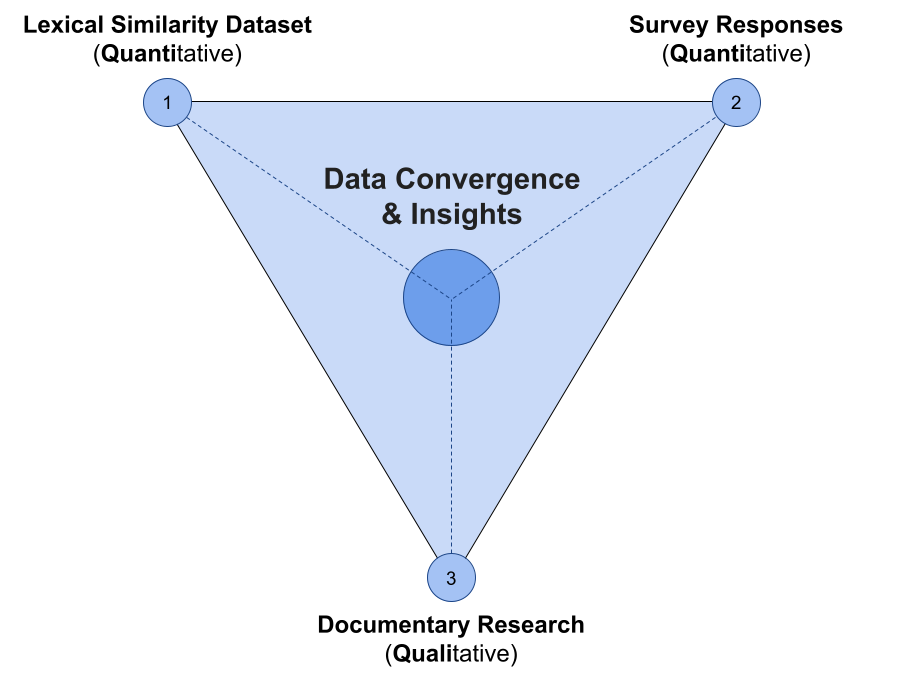
\includegraphics[width=0.77\textwidth]{images/chapter4-cs1-triangulation-sources.png}
\caption{Triangulação de Dados: Fontes de Evidência.}
\label{fig:chap4:triangulation-sources}
\fdireta{FalvoJr2024_FIE}
\end{figure}

A seguir, cada fonte de evidência e suas técnicas de coleta são delineadas, esclarecendo todo o processo de triangulação e sua contribuição para uma compreensão robusta do impacto das tecnologias ASR, como o STT, na acessibilidade educacional.

\subsubsection{1ª Fonte de Evidência: Métodos de Similaridade Léxica}

Esta seção apresenta a metodologia definida para a primeira fonte de evidências da triangulação de dados, onde métodos de similaridade léxica têm como objetivo avaliar e identificar o provedor de ASR/STT mais assertivo para transcrição automática. Nesse sentido, algoritmos de similaridade léxica são métricas particularmente relevantes para a avaliação da precisão de transcrições automáticas, conforme discutido em \citeonline{FalvoJr2023_HICSS}.

Medir a semelhança entre textos é uma prática amplamente investigada em pesquisas acadêmicas, geralmente apoiada por métodos de análise léxica \cite{Majumdar2022}. Para comparar as transcrições automáticas com as de referência é preciso definir como extrair os dados quantitativos por meio de técnicas de similaridade léxica. No contexto deste trabalho de doutorado, e conforme fundamentado anteriormente, destacam-se as seguintes alternativas:

\begin{itemize}

\item \textbf{\sigla{LD}{Distância de Levenshtein}}: Esta métrica de \textit{string} mede a diferença entre duas strings. Basicamente, a LD entre duas palavras é o número mínimo de edições de um único caractere (inserções, exclusões ou substituições) necessárias para transformar uma palavra na outra. Seu nome é uma homenagem a Vladimir Levenshtein, que considerou essa distância em 1965. A comparação LD é geralmente realizada entre duas palavras, determinando o número mínimo de edições necessárias para alterar uma palavra para outra. Quanto maior o número de edições, maior a diferença entre os textos. Uma edição é definida como a inserção, exclusão ou substituição de um caractere \cite{levens-1,levens-2}.

\item \textbf{\sigla{JI}{Índice de Jaccard}}: Esta métrica é definida como a interseção de dois conjuntos de dados dividida pela união desses conjuntos, medindo a similaridade entre eles. No contexto de textos, pode ser expressa como o número de palavras comuns dividido pelo número total de palavras nos dois textos ou documentos. O JI varia de 0 a 1, onde 0 significa nenhuma similaridade e 1 significa sobreposição completa. O JI é calculado dividindo o número de observações em ambos os conjuntos pelo número de observações em cada conjunto, ou seja, o tamanho da interseção dividido pelo tamanho da união de dois conjuntos \cite{jaccard-1,jaccard-2}.

\item \textbf{\sigla{CS}{Similaridade de Cosseno}}: Esta métrica é usada para medir a similaridade entre dois vetores. Especificamente, ela mede a semelhança na direção ou orientação dos vetores, ignorando as diferenças na sua magnitude ou escala. Ambos os vetores devem pertencer ao mesmo espaço de produto interno, o que significa que devem produzir um escalar ao multiplicar o produto interno. A similaridade de dois vetores é medida pelo cosseno do ângulo entre eles. A métrica CS varia de 0 a 1, onde um valor mais próximo de 0 indica menor similaridade e um valor mais próximo de 1 indica maior similaridade \cite{cosseno-1,cosseno-2,cosseno-3}.

\end{itemize}

Neste estudo, foram aplicados os três métodos mencionados, destacando sua relevância. Primeiramente, foram geradas e revisadas as transcrições de referência usando a instância da \textit{Speech2Learning}, desenvolvida como uma POC. Em seguida, cada OA foi transcrito automaticamente utilizando diferentes serviços de ASR/STT, permitindo a comparação entre as transcrições de referência e as automáticas. Dessa forma, foram utilizados os métodos de similaridade léxica CS, JI e LD como métricas de precisão.

Para essa finalidade, foram integrados os principais provedores de ASR/STT baseados em IA do mercado \cite{Gartner2023}: Amazon, Google, IBM, Microsoft e OpenAI. Ademais, em colaboração com a \textit{EdTech} DIO, garantiu-se que o \textit{dataset} deste estudo de caso, devidamente revisado e sintetizado no \autoref{quadro:c4:poc-audios-summary}, estivesse disponível com todas as transcrições de referência dos OAs.

A partir dos áudios do \textit{dataset}, foram integrados os serviços de ASR de cada provedor e geradas suas respectivas transcrições automáticas. Para uma implementação organizada e documentada, utilizou-se o Google Colab, detalhando todo o processo em um primeiro \textit{notebook}\footnote{Colab Notebook - Transcrições Automáticas com ASR/STT: \url{https://bit.ly/S2L-CS1-STTServices}} focado nessas integrações. De forma similar, foram comparadas as 15 transcrições automáticas com as transcrições de referência usando os três métodos de similaridade léxica (CS, JI e LD) em um segundo \textit{notebook}\footnote{Colab Notebook - Algoritmos de Similaridade Léxica: \url{https://bit.ly/S2L-CS1-LexicalAnalysis}}.

\subsubsection{2ª Fonte de Evidência: Respostas do \textit{Survey}}

Como segunda fonte de evidência, foi conduzido um \textit{survey} para avaliar as percepções dos alunos sobre a qualidade das transcrições automáticas fornecidas por ASR/STT. Esta pesquisa, que contou com 56 respostas, coletou \textit{feedback} quantitativo e qualitativo de participantes com experiência em tecnologia e educação. As respostas foram disponibilizadas em \url{https://bit.ly/S2L-CS1-SurveyResp}, bem como uma cópia do formulário no \autoref{appendix:asr-survey} e outra online (\url{https://bit.ly/S2L-CS1-Survey}), garantindo uma compreensão completa dos dados e da dinâmica de preenchimento do questionário.

O \textit{survey} utilizou uma combinação de perguntas de escala Likert e perguntas abertas. As perguntas de escala Likert visavam avaliar quantitativamente a coerência das transcrições automáticas em três idiomas (inglês, português e espanhol). Esta estratégia permitiu uma análise cruzada entre as avaliações técnicas/léxicas e as centradas no usuário. As perguntas abertas buscavam obter \textit{insights} qualitativos sobre a eficácia percebida das soluções de ASR. No entanto, os dados qualitativos não serão analisados nesta fonte de evidência, pois não foram contemplados no projeto original submetido ao CEP e, no contexto deste \textit{survey} predominantemente quantitativo, sua contribuição é limitada.

Os participantes avaliaram as transcrições do mesmo conjunto de 15 videoaulas (cinco por idioma) e dos mesmos cinco provedores (Amazon, Google, IBM, Microsoft e OpenAI) utilizados no estudo de similaridade léxica. Este alinhamento entre as duas fontes garantiu que as respostas do \textit{survey} complementassem diretamente a análise técnica de similaridade léxica, proporcionando uma visão holística do desempenho das transcrições.

Para mitigar possíveis vieses, os provedores foram anonimizados e substituídos por identificadores numéricos aleatórios, garantindo que as avaliações refletissem as experiências genuínas dos usuários, sem influências de preferências por empresas ou marcas, por exemplo. Esta abordagem metodológica está alinhada às melhores práticas em metodologia de pesquisa empírica, conforme defendido por \cite{Sommerville2015}, especialmente na coleta de \textit{feedbacks} e percepções dos usuários em estudos de engenharia de software.

\subsubsection{3ª Fonte de Evidência: Pesquisa Documental}

Para aprofundar a análise dos dados quantitativos, foi realizada uma revisão de literatura que complementa os achados empíricos, identificando estudos relevantes com foco em ASR. Esta revisão oferece uma compreensão mais ampla do potencial e das limitações das tecnologias atuais baseadas em ASR/STT.

Foi utilizada a \textit{Grounded Theory}, ou \sigla{TFD}{Teoria Fundamentada nos Dados}, como um \textit{framework} orientador para a análise documental. A TFD é uma metodologia sistemática e rigorosa utilizada na pesquisa qualitativa para desenvolver teorias emergentes diretamente dos dados \cite{Charmaz2009}. Diferentemente de abordagens que partem de hipóteses preconcebidas, a TFD permite a descoberta de temas e padrões de maneira indutiva, por meio de um processo iterativo de coleta e análise de dados.

Neste estudo, utilizou-se a TFD para examinar os estudos selecionados na pesquisa documental. Este processo incluiu a codificação aberta dos dados, a identificação de temas recorrentes e a integração desses temas em uma teoria coesa. Assim, garantiu-se que as conclusões fossem baseadas diretamente nas evidências coletadas, sem impor noções preconcebidas.

A pesquisa documental envolveu uma revisão complementar da literatura, incluindo artigos, livros e relatórios, focando nas tecnologias ASR e STT no contexto da acessibilidade educacional. Através dessa análise, buscou-se identificar temas recorrentes, diretrizes teóricas e lacunas nas pesquisas existentes, contribuindo para uma compreensão mais detalhada do assunto.

Ao integrar \textit{insights} do conjunto de dados de similaridade lexical, das respostas do \textit{survey} e da pesquisa documental, foi possível fornecer uma visão abrangente e multidimensional do papel do ASR e do STT na melhoria da acessibilidade educacional.

\subsubsection{Triangulação de Dados}

A triangulação, originalmente uma técnica geométrica para determinação de localização, evoluiu para uma metáfora representando métodos de pesquisa que integram diversas abordagens, teorias ou fontes de dados. Essa integração permite uma compreensão mais abrangente de um fenômeno, sendo especialmente útil na pesquisa qualitativa \cite{Yin2015}. 

Segundo \citeonline{Farquhar2020}, a triangulação aumenta a validade de um estudo ao empregar múltiplos métodos para verificar ou corroborar um evento, descrição ou fato específico, reforçando a credibilidade e a confiabilidade da pesquisa. Nesse contexto, os autores ressaltam a importância desse tipo de abordagem aplicada por meio de estudos de caso na indústria.

Neste estudo, adotou-se uma abordagem de triangulação que engloba múltiplas fontes de evidência e suas respectivas técnicas. Esta abordagem de métodos mistos combina resultados qualitativos e quantitativos para aprimorar a análise e a interpretação dos dados coletados. Em particular, a triangulação de dados utiliza várias fontes de evidência para corroborar o mesmo fato ou fenômeno \cite{Yin2015}.

Na Engenharia de Software, a triangulação contribui significativamente para o rigor e a validade da pesquisa. A integração de vários métodos, como pesquisas quantitativas, entrevistas qualitativas e análise documental, permite aos pesquisadores verificar os resultados por meio de uma análise cruzada e obter uma compreensão ainda mais aprofundada de fenômenos complexos. Esta abordagem é particularmente valiosa na análise da eficácia das práticas de desenvolvimento de software, experiência do usuário e adoção de tecnologias \cite{Runeson2009}.

A \autoref{fig:chapter4-cs1-triangulation-methodology} representa a metodologia de triangulação de dados utilizada neste trabalho de doutorado. O diagrama esboça o objeto de estudo, as três fontes distintas de evidência, suas respectivas técnicas de coleta e o processo de convergência de dados que resulta no corpus de dados. Esta abordagem completa e multifacetada garante uma validação robusta e proporciona uma compreensão profunda de como as tecnologias ASR podem melhorar a acessibilidade educacional.

\begin{figure}[htb]
\centering
\caption{Metodologia de Triangulação de Dados Utilizada no Estudo de Caso 1.}
\label{fig:chapter4-cs1-triangulation-methodology}
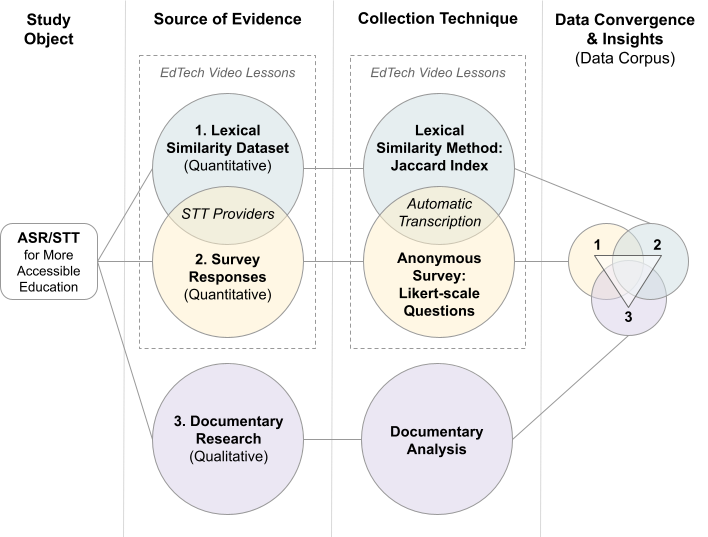
\includegraphics[width=0.9\textwidth]{images/chapter4-cs1-triangulation-methodology.png}
\fdireta{FalvoJr2024_FIE}
\end{figure}

Para as fontes de evidência quantitativas, similaridade léxica e respostas do \textit{survey}, foram estabelecidos dois conjuntos de hipóteses que guiaram as análises. Nesse contexto, hipóteses compartilhadas fazem sentido porque ambas as fontes de evidência exploram as mesmas videoaulas e avaliam os mesmos provedores. Sendo assim, primeiro foi considerada a comparação entre diferentes provedores de transcrição automática, independentemente do idioma. As hipóteses são formuladas da seguinte maneira:

\begin{itemize}
\item \textbf{Hipótese Nula ($H^0$)}: Não há diferença estatisticamente significativa na qualidade das transcrições automáticas entre os provedores.
\item \textbf{Hipótese Alternativa ($H^1$)}: Há uma diferença estatisticamente significativa na qualidade das transcrições automáticas entre os provedores.
\end{itemize}

Em seguida, foi avaliada a qualidade das transcrições automáticas considerando os idiomas Português, Inglês e Espanhol. As hipóteses são delineadas conforme se segue:

\begin{itemize}
\item \textbf{Hipótese Nula ($H^0$)}: Não há diferença estatisticamente significativa na qualidade das transcrições automáticas para Português, Inglês e Espanhol entre os provedores.
\item \textbf{Hipótese Alternativa ($H^1$)}: Há uma diferença estatisticamente significativa na qualidade das transcrições automáticas para Português entre os provedores.
\item \textbf{Hipótese Alternativa ($H^2$)}: Há uma diferença estatisticamente significativa na qualidade das transcrições automáticas para Inglês entre os provedores.
\item \textbf{Hipótese Alternativa ($H^3$)}: Há uma diferença estatisticamente significativa na qualidade das transcrições automáticas para Espanhol entre os provedores.
\end{itemize}

Para a pesquisa documental, adotou-se uma abordagem qualitativa para investigar de maneira mais ampla e exploratória como as tecnologias de reconhecimento de fala para transcrição automática (ASR e STT) influenciam a acessibilidade dos OAs. \textcolor{red}{Essa análise foi orientada pela seguinte questão de pesquisa, que direcionou a investigação deste estudo de caso:}

\begin{citacao}
\textcolor{red}{\textbf{QP do Estudo de Caso 1}: De que maneira as tecnologias de ASR podem contribuir para melhorar a acessibilidade educacional? (\autoref{chapter1:research-questions})}
\end{citacao}

A combinação de hipóteses quantitativas e uma QP qualitativa permitiu uma triangulação robusta de dados, fornecendo uma visão abrangente e multidimensional do impacto das tecnologias de ASR/STT na acessibilidade educacional. A análise das respostas do \textit{survey}, juntamente com os métodos de similaridade léxica e a pesquisa documental, revelou convergências significativas entre as fontes de evidências, enriquecendo as discussões e fortalecendo a validade do estudo como um todo.

Para apresentar uma visão formal, porém simplificada, deste primeiro estudo de caso, o \autoref{quadro:c4:cs1-summary} resume suas principais características. Esta síntese foi elaborada seguindo as diretrizes metodológicas e as perspectivas de pesquisa descritas por \citeonline{CastroFilho2021}, garantindo uma abordagem estruturada e coerente com os padrões de pesquisa científica em informática na educação.

\begin{quadro}[htb]
\centering
\caption{Síntese do Estudo de Caso 1: Legendas Automáticas em Videoaulas}
\label{quadro:c4:cs1-summary}
\begin{tabular}{C{3cm}|m{11.75cm}}\hline
\textbf{Objeto de Estudo} & Serviços de Reconhecimento Automático de Fala (ASR/STT) \\\hline
\textbf{Perspectiva} & Explanatória (Explicativa) \\\hline
\textbf{Característica} & Explicação de causas ou efeitos relacionais ao fenômeno \cite{CastroFilho2021}. \\\hline
\textbf{Objetivos} & \begin{tabular}[c]{@{}m{11.75cm}@{}}1. Avaliar a qualidade das transcrições automáticas fornecidas por diferentes serviços de ASR/STT. \\ 2. Investigar a variação na qualidade das transcrições automáticas em diferentes idiomas (Português, Inglês e Espanhol). \\ 3. Explorar como as transcrições automáticas podem melhorar a acessibilidade educacional.\end{tabular} \\\hline
\textbf{Questões de Pesquisa} & De que maneira as tecnologias de ASR/STT podem contribuir para melhorar a acessibilidade educacional? \\\hline
\textbf{Hipóteses} & \begin{tabular}[c]{@{}m{11.75cm}@{}}1. Existe diferença estatisticamente significativa na precisão das transcrições automáticas entre os provedores de ASR/STT. \\ 2. Existe diferença estatisticamente significativa na precisão das transcrições automáticas para Português, Inglês e Espanhol entre os provedores de ASR/STT.\end{tabular} \\\hline
\textbf{Fontes de Dados} & \begin{tabular}[c]{@{}m{11.75cm}@{}}1. Dados quantitativos de métodos de similaridade léxica (precisão). \\ 2. Respostas quantitativas de um \textit{survey} anônimo (precisão). \\ 3. Dados qualitativos de uma pesquisa documental.\end{tabular} \\\hline
\textbf{Método de Coleta de Dados} & \begin{tabular}[c]{@{}m{11.75cm}@{}}Triangulação de Dados, com as seguintes fontes de evidência: \\ 1. Métodos de similaridade léxica. \\ 2. Respostas do \textit{survey}. \\ 3. Pesquisa documental.\end{tabular} \\\hline
\textbf{Tipo de Análise} & Mista (Quantitativa e Qualitativa) \\\hline
\end{tabular}
\end{quadro}

\subsection{Resultados e Discussões}

\subsubsection{Métodos de Similaridade Léxica}

Com base nas evidências quantitativas, o conjunto de dados projetado para avaliar a qualidade das transcrições automáticas dos principais provedores de ASR (Amazon, Google, IBM, Microsoft e OpenAI) foi analisado por meio de três métricas de similaridade léxica (CS, JI e LD). Dadas as características dos dados coletados, o foco recaiu sobre o JI, única métrica com distribuição normal, demonstrando assim maior robustez estatística. O método de Jaccard, ou Índice de Jaccard, mede a similaridade entre dois conjuntos de dados calculando o tamanho da interseção dividido pelo tamanho da união dos conjuntos de amostras. Logo, ele compara as palavras da transcrição automática com as da transcrição de referência (revisada por especialistas), proporcionando uma medida quantitativa de precisão.

%Sendo assim, vamos apresentar os resultados do JI como métrica principal de similaridade léxica para avaliar os provedores de ASR/STT. 
Os achados iniciais desta fonte de evidência podem ser visualizados por meio do conjunto de gráficos da \autoref{fig:chapter4-cs1-lexical-all}. A figura inclui um Gráfico de Barras (\autoref{fig:chapter4-cs1-lexical-all-barplot}) que exibe o JI médio para cada provedor, um \textit{Boxplot} (\autoref{fig:chapter4-cs1-lexical-all-boxplot}) que detalha a distribuição dos dados e um Gráfico KDE (\autoref{fig:chapter4-cs1-lexical-all-kdeplot}) que ilustra a densidade de probabilidade das pontuações. Essas visualizações destacaram proeminentemente a OpenAI, que demonstrou a maior pontuação, sugerindo seu desempenho superior na captura da similaridade léxica em várias aplicações de transcrição.

\begin{figure}[htbp]
\centering
\caption{Índice de Jaccard: Gráficos dos Provedores Sem Agrupar Por Idioma.}
\label{fig:chapter4-cs1-lexical-all}
\begin{subfigure}[b]{0.8\textwidth}
\centering
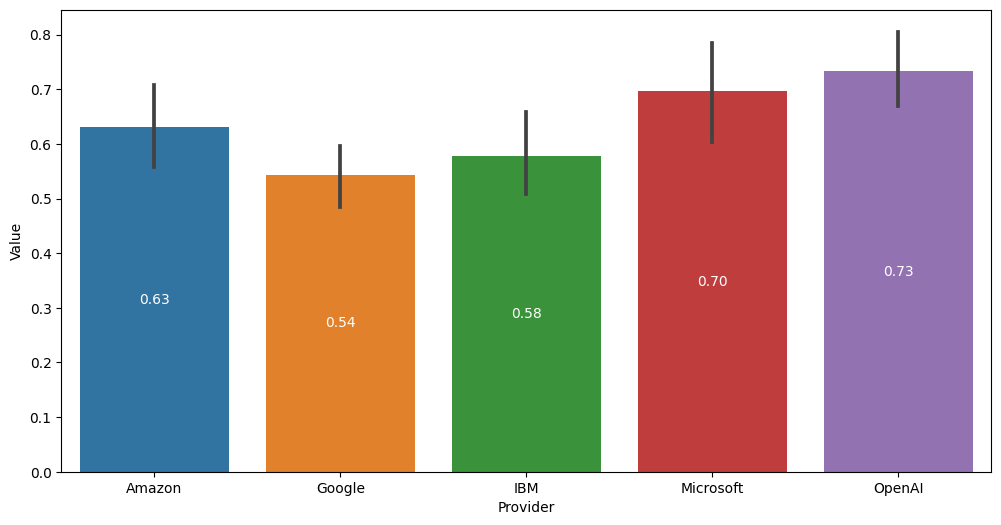
\includegraphics[width=\textwidth]{images/chapter4-cs1-lexical-all-barplot.png}
\caption{Gráfico de Barras.}
\label{fig:chapter4-cs1-lexical-all-barplot}
\end{subfigure} ~
\begin{subfigure}[b]{0.8\textwidth}
\centering
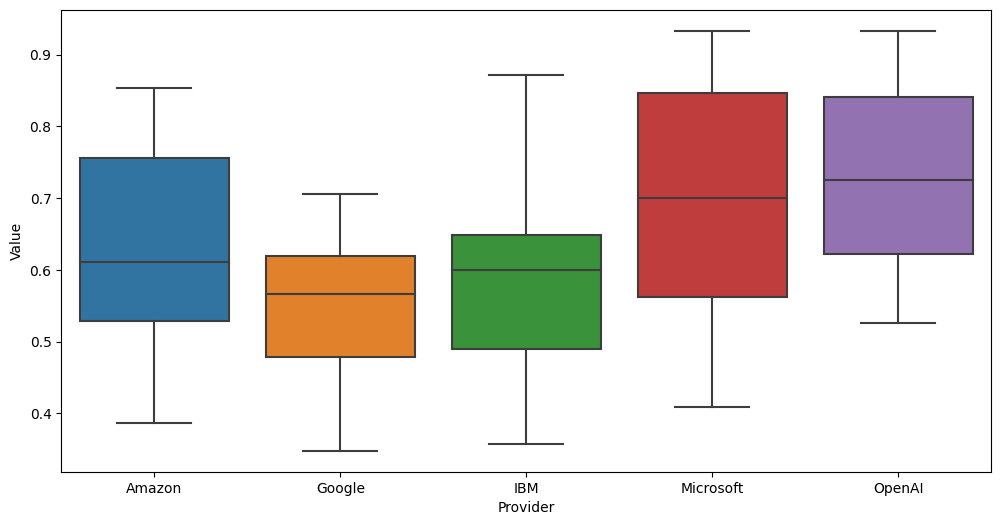
\includegraphics[width=\textwidth]{images/chapter4-cs1-lexical-all-boxplot.png}
\caption{Gráfico de Boxplot.}
\label{fig:chapter4-cs1-lexical-all-boxplot}
\end{subfigure} ~
\begin{subfigure}[b]{0.8\textwidth}
\centering
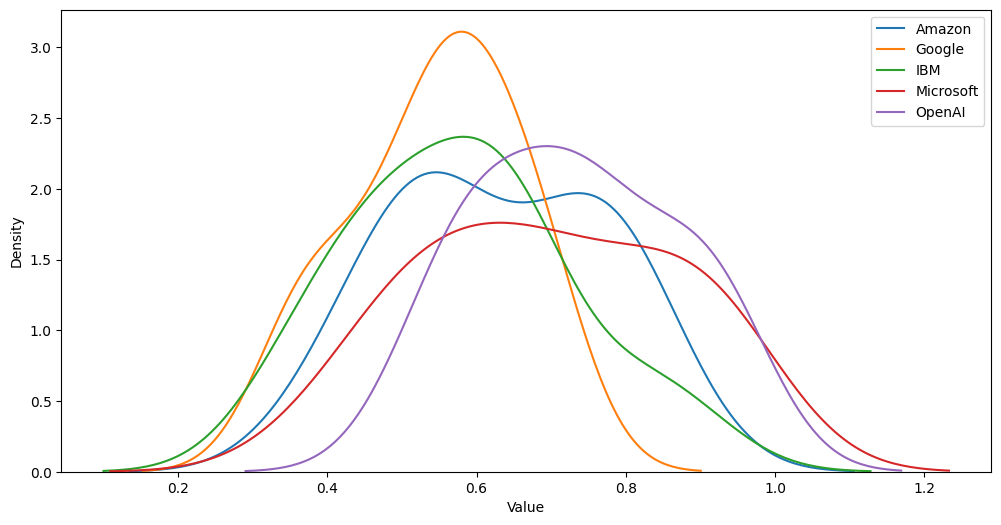
\includegraphics[width=\textwidth]{images/chapter4-cs1-lexical-all-kdeplot.png}
\caption{Gráfico KDE.}
\label{fig:chapter4-cs1-lexical-all-kdeplot}
\end{subfigure}
\fdireta{FalvoJr2023_HICSS}
\end{figure}

As análises estatísticas detalhadas na \autoref{tabble:c4:results-ji-tests} corroboram as impressões iniciais dos gráficos. Os testes de normalidade, o \textit{Kolmogorov-Smirnov} \cite{Kolmogorov1933,Smirnov1948} e o \textit{Shapiro-Wilk} \cite{Shapiro1965}, confirmaram a distribuição normal dos dados, permitindo uma análise adicional por meio da \textit{One-Way ANOVA} \cite{Fisher1925}. 

Por sua vez, o teste de ANOVA revelou diferenças significativas entre os provedores. Portanto, as análises \textit{post-hoc} de \textit{Tukey HSD} \cite{Tukey1949} e de \textit{Bonferroni} \cite{Bonferroni1936} foram aplicadas para identificar essas diferenças explicitamente. 

\begin{table}[htb]
\small
\centering
\caption{Testes Estatísticos do Índice de Jaccard: Provedores Sem Agrupar Por Idioma}
\label{tabble:c4:results-ji-tests} 
\begin{tabular}{lcclc|}
\hline
\multicolumn{5}{|c|}{\textbf{Tests of Normality}} \\ \hline
\multicolumn{1}{|c|}{\multirow{2}{*}{\textbf{Test}}} & \multicolumn{2}{c|}{\textbf{Kolmogorov-Smirnov}} & \multicolumn{2}{c|}{\textbf{Shapiro-Wilk}} \\ \cline{2-5} 
\multicolumn{1}{|c|}{} & \multicolumn{1}{c|}{\textbf{Statistic}} & \multicolumn{1}{c|}{\textbf{Significance \ensuremath{(p)}}} & \multicolumn{1}{c|}{\textbf{Statistic}} & \textbf{\ensuremath{p}} \\ \hline
\multicolumn{1}{|c|}{Jaccard Index} & \multicolumn{1}{c|}{0.057} & \multicolumn{1}{c|}{\textbf{0.200}} & \multicolumn{1}{c|}{0.973} & \textbf{0.111} \\ \hline
\multicolumn{5}{|c|}{\textbf{Interpretation}} \\ \hline
\multicolumn{5}{|l|}{\begin{tabular}[c]{@{}l@{}}Kolmogorov-Smirnov: If \ensuremath{p>0.05}, sample follow the same statistical distribution.\end{tabular}} \\ \hline
\multicolumn{5}{|l|}{Shapiro-wilk: If \ensuremath{p>0.05} is normal.} \\ \hline
\multicolumn{5}{|c|}{\textbf{One-Way ANOVA (One-Way Analysis of Variance)}} \\ \hline
\multicolumn{1}{|c|}{\textbf{Test}} & \multicolumn{2}{c|}{\textbf{F}} & \multicolumn{2}{c|}{\textbf{\ensuremath{p}}} \\ \hline
\multicolumn{1}{|c|}{Jaccard Index} & \multicolumn{2}{c|}{4.562} & \multicolumn{2}{c|}{\textbf{0.002}} \\ \hline
\multicolumn{5}{|c|}{\textbf{Interpretation}} \\ \hline
\multicolumn{5}{|l|}{\begin{tabular}[c]{@{}l@{}}If \ensuremath{p<0.05}, there are significant differences between at least two groups.\end{tabular}} \\ \hline
\multicolumn{5}{|c|}{\textbf{Tukey HSD (Honest Significant Difference)}} \\ \hline
\multicolumn{3}{|l|}{\textbf{Providers (Groups from 1 to 5)}} & \multicolumn{2}{c|}{\textbf{\ensuremath{p}}} \\ \hline
\multicolumn{3}{|l|}{OpenAI (Group 5) to Google (Group 2)} & \multicolumn{2}{c|}{\textbf{0.005}} \\ \hline
\multicolumn{3}{|l|}{OpenAI (Group 5) to IBM (Group 3)} & \multicolumn{2}{c|}{\textbf{0.032}} \\ \hline
\multicolumn{3}{|l|}{Microsoft (Group 4) to Google (Group 2)} & \multicolumn{2}{c|}{\textbf{0.037}} \\ \hline
\multicolumn{5}{|c|}{\textbf{Interpretation}} \\ \hline
\multicolumn{5}{|l|}{\begin{tabular}[c]{@{}l@{}}If \ensuremath{p<>0} and \ensuremath{p<0.05}, there is a significant difference among the groups.\end{tabular}} \\ \hline
\multicolumn{5}{|c|}{\textbf{Bonferroni}} \\ \hline
\multicolumn{3}{|l|}{\textbf{Providers (Groups from 1 to 5)}} & \multicolumn{2}{c|}{\textbf{\ensuremath{p}}} \\ \hline
\multicolumn{3}{|l|}{OpenAI (Group 5) to Google (Group 2)} & \multicolumn{2}{c|}{\textbf{0.006}} \\ \hline
\multicolumn{3}{|l|}{OpenAI (Group 5) to IBM (Group 3)} & \multicolumn{2}{c|}{\textbf{0.041}} \\ \hline
\multicolumn{3}{|l|}{Microsoft (Group 4) to Google (Group 2)} & \multicolumn{2}{c|}{\textbf{0.047}} \\ \hline
\multicolumn{5}{|c|}{\textbf{Interpretation}} \\ \hline
\multicolumn{5}{|l|}{\begin{tabular}[c]{@{}l@{}}If the adjusted \ensuremath{p~(\alpha'=\alpha/n)}, where n is the number of comparisons, is \ensuremath{<0.05},\\then there is a statistical difference among the groups.\end{tabular}} \\ \hline
\end{tabular}
\fdireta{FalvoJr2023_HICSS}
\end{table}

Adicionalmente, tendo em vista os dois conjuntos de hipóteses de pesquisa, as análises foram estendidas para avaliar o desempenho dos provedores em múltiplos idiomas: Português, Inglês e Espanhol (\autoref{fig:chapter4-cs1-lexical-by-lang-barplot}). Esta segmentação linguística revelou disparidades de precisão persistentes, que são críticas para aplicações globais que dependem de transcrições automáticas confiáveis em várias línguas.

\begin{figure}[htb]
\centering
\caption{Índice de Jaccard: Gráfico dos Provedores Agrupados Por Idioma.}
\label{fig:chapter4-cs1-lexical-by-lang-barplot}
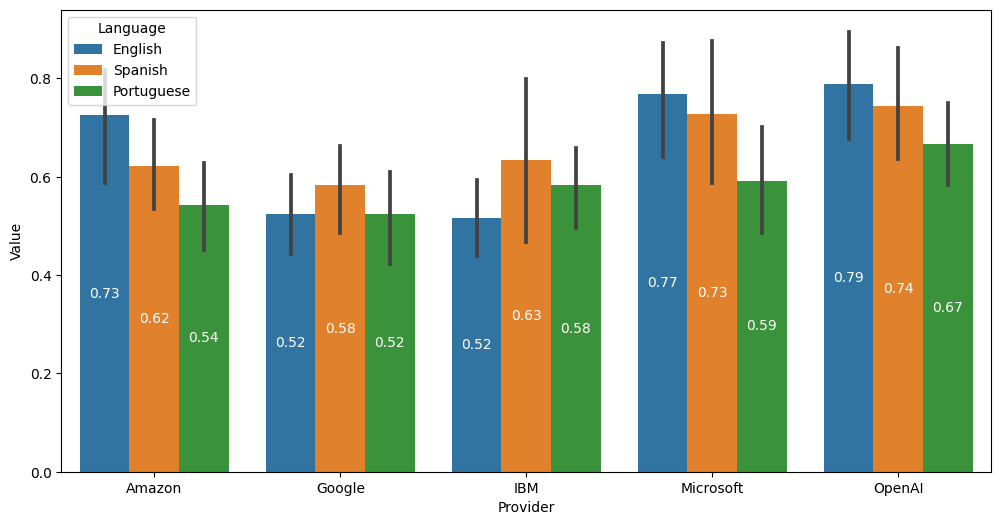
\includegraphics[width=0.9\textwidth]{images/chapter4-cs1-lexical-by-lang-barplot.png}
\fdireta{FalvoJr2023_HICSS}
\end{figure}

Como resultado, foram identificadas diferenças estatisticamente significativas entre a OpenAI quando comparada com Google e IBM, além da Microsoft quando comparada ao Google. Essas diferenças evidenciam uma variabilidade na eficiência dos provedores ao lidar com a similaridade léxica em diferentes contextos de transcrição automática, sugerindo uma superioridade da OpenAI e da Microsoft tendo em vista suas medidas de Jaccard.

As avaliações estatísticas correspondentes (\autoref{table:c4:results-ji-by-lang-tests}) incluíram testes de normalidade e \textit{One-Way ANOVA} para cada idioma. Os resultados destacaram diferenças significativas em como os provedores geram transcrições automáticas em inglês. Disparidades específicas entre provedores foram detalhadas através de análises \textit{post-hoc}, como \textit{Tukey HSD} e \textit{Bonferroni} para o idioma inglês, indicando que o desempenho pode variar significativamente dependendo do idioma das transcrições.

\begin{table}[htb]
\small
\centering
\caption{Testes Estatísticos do Índice de Jaccard: Provedores Agrupados Por Idioma}
\label{table:c4:results-ji-by-lang-tests} 
\begin{tabular}{|ccccc|}
\hline
\multicolumn{5}{|c|}{\textbf{Tests of Normality}} \\ \hline
\multicolumn{1}{|c|}{\multirow{2}{*}{\textbf{Test}}} & \multicolumn{2}{c|}{\textbf{Kolmogorov-Smirnov}} & \multicolumn{2}{c|}{\textbf{Shapiro-Wilk}} \\ \cline{2-5} 
\multicolumn{1}{|c|}{} & \multicolumn{1}{c|}{\textbf{Statistic}} & \multicolumn{1}{c|}{\textbf{Significance \ensuremath{(p)}}} & \multicolumn{1}{c|}{\textbf{Statistic}} & \textbf{\ensuremath{p}} \\ \hline
\multicolumn{1}{|c|}{EN} & \multicolumn{1}{c|}{0.121} & \multicolumn{1}{c|}{\textbf{0.200}} & \multicolumn{1}{c|}{0.961} & \textbf{0.427} \\ \hline
\multicolumn{1}{|c|}{PT} & \multicolumn{1}{c|}{0.114} & \multicolumn{1}{c|}{\textbf{0.200}} & \multicolumn{1}{c|}{0.942} & \textbf{0.169} \\ \hline
\multicolumn{1}{|c|}{ES} & \multicolumn{1}{c|}{0.951} & \multicolumn{1}{c|}{\textless 0.001} & \multicolumn{1}{c|}{0.951} & \textbf{0.264} \\ \hline
\multicolumn{5}{|c|}{\textbf{One-Way ANOVA}} \\ \hline
\multicolumn{1}{|c|}{\textbf{Test}} & \multicolumn{2}{c|}{\textbf{F}} & \multicolumn{2}{c|}{\textbf{\ensuremath{p}}} \\ \hline
\multicolumn{1}{|c|}{EN} & \multicolumn{2}{c|}{4.88} & \multicolumn{2}{c|}{\textbf{0.007}} \\ \hline
\multicolumn{1}{|c|}{PT} & \multicolumn{2}{c|}{1.058} & \multicolumn{2}{c|}{0.403} \\ \hline
\multicolumn{1}{|c|}{ES} & \multicolumn{2}{c|}{0,931} & \multicolumn{2}{c|}{0,466} \\ \hline
\multicolumn{5}{|c|}{\textbf{Tukey HSD (Honest Significant Difference) - EN}} \\ \hline
\multicolumn{3}{|l|}{\textbf{Providers (Groups from 1 to 5)}} & \multicolumn{2}{c|}{\textbf{\ensuremath{p}}} \\ \hline
\multicolumn{3}{|l|}{OpenAI (Group 5) to Google (Group 2)} & \multicolumn{2}{c|}{\textbf{0.041}} \\ \hline
\multicolumn{3}{|l|}{OpenAI (Group 5) to IBM (Group 3)} & \multicolumn{2}{c|}{\textbf{0.034}} \\ \hline
\multicolumn{5}{|c|}{\textbf{Bonferroni - EN}} \\ \hline
\multicolumn{3}{|l|}{\textbf{Providers (Groups from 1 to 5)}} & \multicolumn{2}{c|}{\textbf{\ensuremath{p}}} \\ \hline
\multicolumn{3}{|l|}{OpenAI (Group 5) to IBM (Group 3)} & \multicolumn{2}{c|}{\textbf{0.047}} \\ \hline
\end{tabular}
\fdireta{FalvoJr2023_HICSS}
\end{table}

Esses resultados destacam diferenças significativas na qualidade das transcrições automáticas dos provedores avaliados em relação à similaridade léxica. Além disso, abrem caminho para uma exploração mais aprofundada de como essas características podem impactar a experiência do usuário em várias aplicações dessas transcrições. Isso inclui a satisfação do aluno e a percepção sobre a precisão da transcrição em diferentes contextos linguísticos. Tais aspectos são discutidos a seguir, com base nos resultados do \textit{survey}.

\subsubsection{Respostas do \textit{Survey}}

Com base nos \textit{insights} do estudo de similaridade léxica, esta seção apresenta os resultados de uma pesquisa anônima baseada nas percepções dos participantes sobre a qualidade das transcrições automáticas, explorando o \textit{dataset} definido para as fontes de evidência quantitativas. Essa pesquisa teve como objetivo comparar os dados objetivos de similaridade léxica com as avaliações subjetivas de pessoas reais sobre a qualidade das transcrições dos diferentes provedores de serviços de ASR/STT.

Os resultados foram sintetizados na \autoref{fig:chapter4-cs1-survey-all}, ilustrando as avaliações médias e a distribuição das respostas. O gráfico de barras (\autoref{fig:chapter4-cs1-survey-all-barplot}) apresenta as avaliações médias para cada provedor, com a OpenAI recebendo a maior pontuação, o que sugere uma preferência entre os participantes. O gráfico de \textit{boxplot} (\autoref{fig:chapter4-cs1-survey-all-boxplot}) detalha a dispersão e a tendência central das avaliações para cada provedor, evidenciando a variação na satisfação dos usuários, enquanto o gráfico KDE (\autoref{fig:chapter4-cs1-survey-all-kdeplot}) oferece uma estimativa visual da densidade da distribuição das avaliações.

\begin{figure}[htbp]
\centering
\caption{Respostas do \textit{Survey}: Gráficos dos Provedores Sem Agrupar Por Idioma.}
\label{fig:chapter4-cs1-survey-all}
\begin{subfigure}[b]{0.77\textwidth}
\centering
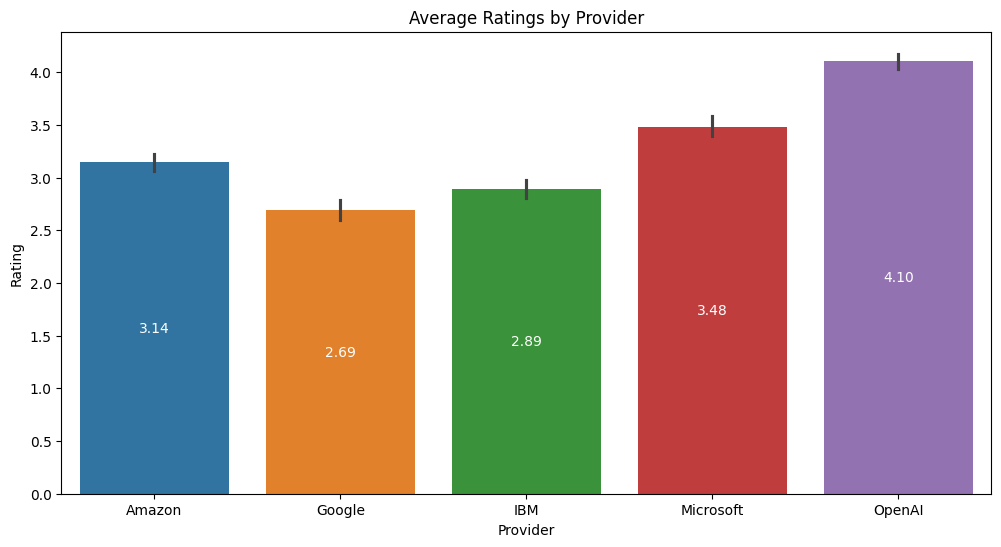
\includegraphics[width=\textwidth]{images/chapter4-cs1-survey-all-barplot.png}
\caption{Gráfico de Barras.}
\label{fig:chapter4-cs1-survey-all-barplot}
\end{subfigure} ~
\begin{subfigure}[b]{0.77\textwidth}
\centering
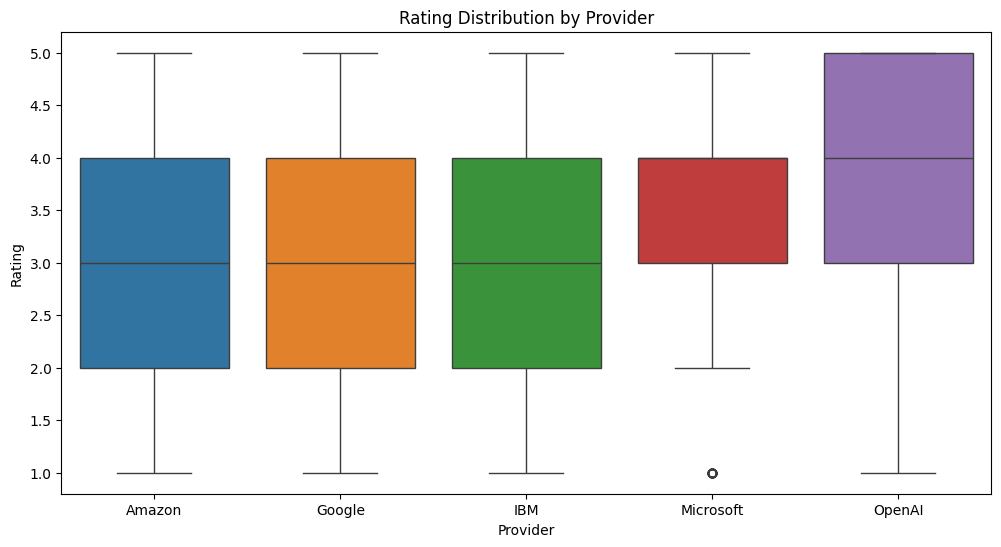
\includegraphics[width=\textwidth]{images/chapter4-cs1-survey-all-boxplot.png}
\caption{Gráfico de Boxplot.}
\label{fig:chapter4-cs1-survey-all-boxplot}
\end{subfigure} ~
\begin{subfigure}[b]{0.77\textwidth}
\centering
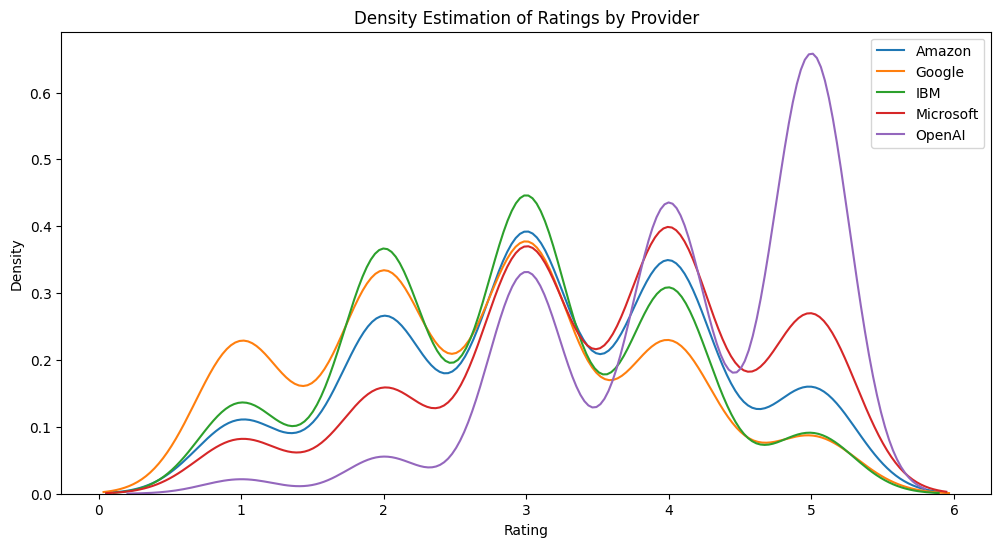
\includegraphics[width=\textwidth]{images/chapter4-cs1-survey-all-kdeplot.png}
\caption{Gráfico KDE.}
\label{fig:chapter4-cs1-survey-all-kdeplot}
\end{subfigure}
\fdireta{FalvoJr2024_FIE}
\end{figure}

Um gráfico adicional detalha as avaliações por idioma, indicando variações significativas na satisfação do usuário com base no idioma da transcrição automática (\autoref{fig:chapter4-cs1-survey-by-lang-barplot}), o que pode sugerir níveis de qualidade distintos para transcrições em Português, Inglês ou Espanhol.

\begin{figure}[htb]
\centering
\caption{Respostas do \textit{Survey}: Gráfico dos Provedores Agrupados Por Idioma.}
\label{fig:chapter4-cs1-survey-by-lang-barplot}
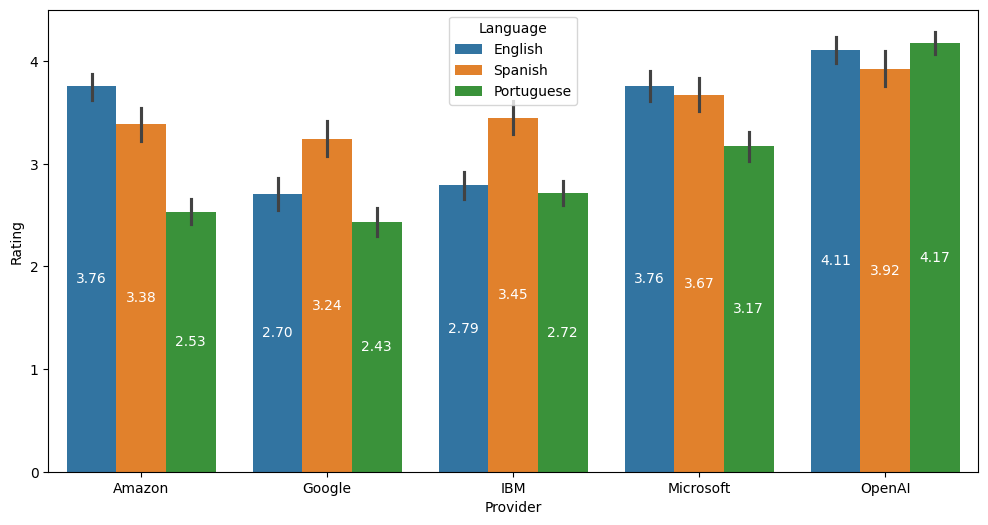
\includegraphics[width=1\textwidth]{images/chapter4-cs1-survey-by-lang-barplot.png}
\fdireta{FalvoJr2024_FIE}
\end{figure}

As análises estatísticas, consolidadas na \autoref{table:c4:results-survey-tests}, indicaram que as respostas do \textit{survey} não seguiram uma distribuição normal, característica confirmada pelos testes de \textit{Kolmogorov-Smirnov} \cite{Kolmogorov1933,Smirnov1948} e \textit{Shapiro-Wilk} \cite{Shapiro1965}. Nesse sentido, fez-se necessário a avaliação e aplicação de testes não paramétricos para as análises subsequentes. O teste de \textit{Kruskal-Wallis} \cite{Kruskal1952}, uma alternativa não paramétrica ao ANOVA, foi empregado para determinar se havia diferenças significativas nas medianas das pontuações entre os diferentes grupos. Este teste mostrou diferenças significativas entre os provedores (\ensuremath{p < 0.05}), sugerindo que as percepções dos participantes variavam significativamente dependendo do provedor.

Ainda analisando a \autoref{table:c4:results-survey-tests}, dada a distribuição não normal dos dados, o teste de \textit{Dunn} \cite{Dunn1964} foi escolhido em detrimento do teste de \textit{Conover} \cite{Conover1999} para a análise \textit{post-hoc} devido às suas suposições menos rigorosas sobre a distribuição dos dados e sua capacidade de lidar efetivamente com dados que possuem \textit{outliers}, embora ambos tenham produzido resultados análogos em testes informais. O teste de \textit{Dunn} comparou pares de provedores, indicando diferenças significativas entre quase todos os pares. Notavelmente, todas as comparações envolvendo OpenAI e outros provedores demonstraram diferenças significativas, sugerindo uma virtual superioridade desse provedor.

\begin{table}[htb]
\small
\centering
\caption{Testes Estatísticos do \textit{Survey}: Provedores Sem Agrupar Por Idioma}
\label{table:c4:results-survey-tests} 
\begin{tabular}{|lcccc|}
\hline
\multicolumn{5}{|c|}{\textbf{Tests of Normality}} \\ \hline
\multicolumn{1}{|c|}{\multirow{2}{*}{\textbf{Test}}} & \multicolumn{2}{c|}{\textbf{Kolmogorov-Smirnov}} & \multicolumn{2}{c|}{\textbf{Shapiro-Wilk}} \\ \cline{2-5} 
\multicolumn{1}{|c|}{} & \multicolumn{1}{c|}{\textbf{Statistic}} & \multicolumn{1}{c|}{\textbf{Significance \ensuremath{(p)}}} & \multicolumn{1}{c|}{\textbf{Statistic}} & \textbf{\ensuremath{p}} \\ \hline
\multicolumn{1}{|c|}{Survey Responses} & \multicolumn{1}{c|}{0.887} & \multicolumn{1}{c|}{\textless 0.001} & \multicolumn{1}{c|}{0.973} & \textless 0.001 \\ \hline
\multicolumn{5}{|c|}{\textbf{Interpretation}} \\ \hline
\multicolumn{5}{|l|}{\begin{tabular}[c]{@{}l@{}}Kolmogorov-Smirnov: If \ensuremath{p>0.05}, sample follow the same  statistical distribution.\end{tabular}} \\ \hline
\multicolumn{5}{|l|}{Shapiro-wilk: If \ensuremath{p>0.05} is normal.} \\ \hline
\multicolumn{5}{|c|}{\textbf{Kruskal-Wallis (Non-Parametric equivalent to ANOVA)}} \\ \hline
\multicolumn{1}{|c|}{\textbf{Test}} & \multicolumn{2}{c|}{\textbf{Statistic}} & \multicolumn{2}{c|}{\textbf{\ensuremath{p}}} \\ \hline
\multicolumn{1}{|c|}{Survey Responses} & \multicolumn{2}{c|}{536.167} & \multicolumn{2}{c|}{\textbf{\textless 0.001}} \\ \hline
\multicolumn{5}{|c|}{\textbf{Interpretation}} \\ \hline
\multicolumn{5}{|l|}{\begin{tabular}[c]{@{}l@{}}If \ensuremath{p<0.05}, there are significant differences among the groups.\end{tabular}} \\ \hline
\multicolumn{5}{|c|}{\textbf{Dunn (Non-Parametric Post-Hoc equivalent to Tukey HSB)}} \\ \hline
\multicolumn{3}{|l|}{\textbf{Providers (Groups from 1 to 5)}} & \multicolumn{2}{c|}{\textbf{\ensuremath{p}}} \\ \hline
\multicolumn{3}{|l|}{Amazon (Group 1) to Google (Group 2)} & \multicolumn{2}{c|}{\textbf{\textless 0.001}} \\ \hline
\multicolumn{3}{|l|}{Amazon (Group 1) to IBM (Group 3)} & \multicolumn{2}{c|}{\textbf{\textless 0.001}} \\ \hline
\multicolumn{3}{|l|}{Amazon (Group 1) to Micorsoft (Group 4)} & \multicolumn{2}{c|}{\textbf{\textless 0.001}} \\ \hline
\multicolumn{3}{|l|}{Amazon (Group 1) to OpenAI (Group 5)} & \multicolumn{2}{c|}{\textbf{\textless 0.001}} \\ \hline
\multicolumn{3}{|l|}{Google (Group 2) to IBM (Group 3)} & \multicolumn{2}{c|}{\textbf{0.010}} \\ \hline
\multicolumn{3}{|l|}{Google (Group 2) to Microsoft (Group 4)} & \multicolumn{2}{c|}{\textbf{\textless 0.001}} \\ \hline
\multicolumn{3}{|l|}{Google (Group 2) to OpenAI (Group 5)} & \multicolumn{2}{c|}{\textbf{\textless 0.001}} \\ \hline
\multicolumn{3}{|l|}{IBM (Group 3) to Microsoft (Group 4)} & \multicolumn{2}{c|}{\textbf{\textless 0.001}} \\ \hline
\multicolumn{3}{|l|}{IBM (Group 3) to OpenAI (Group 5)} & \multicolumn{2}{c|}{\textbf{\textless 0.001}} \\ \hline
\multicolumn{3}{|l|}{Micorsoft (Group 4) to OpenAI (Group 5)} & \multicolumn{2}{c|}{\textbf{\textless 0.001}} \\ \hline
\multicolumn{5}{|c|}{\textbf{Interpretation}} \\ \hline
\multicolumn{5}{|l|}{\begin{tabular}[c]{@{}l@{}}If \ensuremath{p<0.05}, it indicates significant pairwise differences between groups.\end{tabular}} \\ \hline
\end{tabular}
\fdireta{FalvoJr2024_FIE}
\end{table}

Os resultados estratificados por idioma reforçaram essas descobertas, com todos os grupos de idiomas mostrando diferenças significativas entre os provedores na forma como as transcrições automáticas foram avaliadas. Isso sugere que a qualidade percebida pelos participantes não depende apenas do provedor, mas também varia com o idioma, destacando os desafios de fornecer transcrições de alta qualidade de forma uniforme em diferentes contextos linguísticos (\autoref{table:c4:results-survey-by-lang-tests}).

\begin{table}[htb]
\small
\centering
\caption{Testes Estatísticos do \textit{Survey}: Provedores Agrupados Por Idioma}
\label{table:c4:results-survey-by-lang-tests} 
\begin{tabular}{|lcccc|}
\hline
\multicolumn{5}{|c|}{\textbf{Tests of Normality}} \\ \hline
\multicolumn{1}{|c|}{\multirow{2}{*}{\textbf{Test}}} & \multicolumn{2}{c|}{\textbf{Kolmogorov-Smirnov}} & \multicolumn{2}{c|}{\textbf{Shapiro-Wilk}} \\ \cline{2-5} 
\multicolumn{1}{|c|}{} & \multicolumn{1}{c|}{\textbf{Statistic}} & \multicolumn{1}{c|}{\textbf{Significance \ensuremath{(p)}}} & \multicolumn{1}{c|}{\textbf{Statistic}} & \textbf{\ensuremath{p}} \\ \hline
\multicolumn{1}{|c|}{EN} & \multicolumn{1}{c|}{0.897} & \multicolumn{1}{c|}{\textless 0.001} & \multicolumn{1}{c|}{0.897} & \textless 0.001 \\ \hline
\multicolumn{1}{|c|}{PT} & \multicolumn{1}{c|}{0.847} & \multicolumn{1}{c|}{\textless 0.001} & \multicolumn{1}{c|}{0.912} & \textless 0.001 \\ \hline
\multicolumn{1}{|c|}{ES} & \multicolumn{1}{c|}{0.959} & \multicolumn{1}{c|}{\textless 0.001} & \multicolumn{1}{c|}{0.893} & \textless 0.001 \\ \hline
\multicolumn{5}{|c|}{\textbf{Kruskal-Wallis (Non-Parametric)}} \\ \hline
\multicolumn{1}{|c|}{\textbf{Test}} & \multicolumn{2}{c|}{\textbf{Statistic}} & \multicolumn{2}{c|}{\textbf{\ensuremath{p}}} \\ \hline
\multicolumn{1}{|c|}{EN} & \multicolumn{2}{c|}{244.355} & \multicolumn{2}{c|}{\textbf{\textless 0.001}} \\ \hline
\multicolumn{1}{|c|}{PT} & \multicolumn{2}{c|}{355.323} & \multicolumn{2}{c|}{\textbf{\textless 0.001}} \\ \hline
\multicolumn{1}{|c|}{ES} & \multicolumn{2}{c|}{37.615} & \multicolumn{2}{c|}{\textbf{\textless 0.001}} \\ \hline
\multicolumn{5}{|c|}{\textbf{Dunn (Non-Parametric) - EN}} \\ \hline
\multicolumn{3}{|l|}{\textbf{Providers (Groups from 1 to 5)}} & \multicolumn{2}{c|}{\textbf{\ensuremath{p}}} \\ \hline
\multicolumn{3}{|l|}{Amazon (Group 1) to Google (Group 2)} & \multicolumn{2}{c|}{\textbf{\textless 0.001}} \\ \hline
\multicolumn{3}{|l|}{Amazon (Group 1) to IBM (Group 3)} & \multicolumn{2}{c|}{\textbf{\textless 0.001}} \\ \hline
\multicolumn{3}{|l|}{Amazon (Group 1) to OpenAI (Group 5)} & \multicolumn{2}{c|}{\textbf{0.002}} \\ \hline
\multicolumn{3}{|l|}{Google (Group 2) to Microsoft (Group 4)} & \multicolumn{2}{c|}{\textbf{\textless 0.001}} \\ \hline
\multicolumn{3}{|l|}{Google (Group 2) to OpenAI (Group 5)} & \multicolumn{2}{c|}{\textbf{\textless 0.001}} \\ \hline
\multicolumn{3}{|l|}{IBM (Group 3) to Microsoft (Group 4)} & \multicolumn{2}{c|}{\textbf{\textless 0.001}} \\ \hline
\multicolumn{3}{|l|}{IBM (Group 3) to OpenAI (Group 5)} & \multicolumn{2}{c|}{\textbf{\textless 0.001}} \\ \hline
\multicolumn{3}{|l|}{Micorsoft (Group 4) to OpenAI (Group 5)} & \multicolumn{2}{c|}{\textbf{0.005}} \\ \hline
\multicolumn{5}{|c|}{\textbf{Dunn (Non-Parametric) - PT}} \\ \hline
\multicolumn{3}{|l|}{\textbf{Providers (Groups from 1 to 5)}} & \multicolumn{2}{c|}{\textbf{\ensuremath{p}}} \\ \hline
\multicolumn{3}{|l|}{Amazon (Group 1) to Microsoft (Group 4)} & \multicolumn{2}{c|}{\textbf{\textless 0.001}} \\ \hline
\multicolumn{3}{|l|}{Amazon (Group 1) to OpenAI (Group 5)} & \multicolumn{2}{c|}{\textbf{\textless 0.001}} \\ \hline
\multicolumn{3}{|l|}{Google (Group 2) to IBM (Group 3)} & \multicolumn{2}{c|}{\textbf{0.017}} \\ \hline
\multicolumn{3}{|l|}{Google (Group 2) to Microsoft (Group 4)} & \multicolumn{2}{c|}{\textbf{\textless 0.001}} \\ \hline
\multicolumn{3}{|l|}{Google (Group 2) to OpenAI (Group 5)} & \multicolumn{2}{c|}{\textbf{\textless 0.001}} \\ \hline
\multicolumn{3}{|l|}{IBM (Group 3) to Microsoft (Group 4)} & \multicolumn{2}{c|}{\textbf{\textless 0.001}} \\ \hline
\multicolumn{3}{|l|}{IBM (Group 3) to OpenAI (Group 5)} & \multicolumn{2}{c|}{\textbf{\textless 0.001}} \\ \hline
\multicolumn{3}{|l|}{Micorsoft (Group 4) to OpenAI (Group 5)} & \multicolumn{2}{c|}{\textbf{\textless 0.001}} \\ \hline
\multicolumn{5}{|c|}{\textbf{Dunn (Non-Parametric) - ES}} \\ \hline
\multicolumn{3}{|l|}{\textbf{Providers (Groups from 1 to 5)}} & \multicolumn{2}{c|}{\textbf{\ensuremath{p}}} \\ \hline
\multicolumn{3}{|l|}{Amazon (Group 1) to OpenAI (Group 5)} & \multicolumn{2}{c|}{\textbf{\textless 0.001}} \\ \hline
\multicolumn{3}{|l|}{Google (Group 2) to Microsoft (Group 4)} & \multicolumn{2}{c|}{\textbf{0.002}} \\ \hline
\multicolumn{3}{|l|}{Google (Group 2) to OpenAI (Group 5)} & \multicolumn{2}{c|}{\textbf{\textless 0.001}} \\ \hline
\multicolumn{3}{|l|}{IBM (Group 3) to OpenAI (Group 5)} & \multicolumn{2}{c|}{\textbf{\textless 0.001}} \\ \hline
\end{tabular}
\fdireta{FalvoJr2024_FIE}
\end{table}

A análise da pesquisa efetivamente conecta as medidas objetivas de similaridade léxica e as percepções subjetivas da qualidade das transcrições. A correlação entre as pontuações de similaridade léxica e as excelentes avaliações dos participantes, particularmente para a OpenAI, ressalta a relevância prática da precisão léxica na satisfação dos usuários finais. 

Esses \textit{insights} são fundamentais para provedores que buscam otimizar seus serviços de transcrição para conteúdos educacionais, pois ilustram a importância tanto da precisão linguística quanto da percepção dos usuários finais na avaliação da qualidade das transcrições automáticas. As descobertas sugerem um roteiro para futuras melhorias e a potencial customização de serviços para atender de forma mais eficaz às diversas necessidades linguísticas.

\subsubsection{Pesquisa Documental}

Nesta fase, ampliou-se a visão sobre as tecnologias de ASR/STT, examinando a literatura para complementar as descobertas quantitativas com percepções qualitativas adicionais. Esta análise documental aprofunda-se em diversos estudos que contribuíram significativamente para o campo do ASR, proporcionando uma compreensão mais ampla de como essas tecnologias, impulsionadas por avanços em \textit{Machine Learning} (ML) e IA, podem tornar OAs mais acessíveis.

O estudo de \citeonline{Ferraro2023} apresenta uma investigação extensa sobre a transcrição de língua falada usando modelos de ML. Sua análise compara serviços de STT de código aberto e pagos, com foco na qualidade das transcrições automáticas e na diversidade dos dados de entrada. A pesquisa utiliza diversos conjuntos de dados de entrevistas, palestras e discursos, empregando métricas como a WER para avaliação. O trabalho de \citeonline{Ferraro2023} fornece um ponto de referência, alternativo aos métodos de similaridade léxica, para avaliar a precisão da transcrição, estabelecendo uma base sólida para trabalhos futuros.

\citeonline{Bengesi2024} oferecem uma revisão abrangente dos avanços recentes em IAGen, destacando suas aplicações potenciais em processos automáticos de transcrição. Embora não se concentrem diretamente na conversão de fala em texto, sua exploração de modelos de ponta, incluindo Redes Adversárias Generativas (GANs), Transformadores Pré-treinados Generativos (GPT), \textit{autoencoders} e modelos de difusão, fornece uma base para entender como a IAGen pode aprimorar a precisão da transcrição.

\citeonline{Homburg2019} exploram o uso de robôs humanoides como avatares para a tradução de língua de sinais, buscando aprimorar a inclusão da comunidade surda. Diferentemente de pesquisas anteriores, que se concentravam apenas no reconhecimento da língua de sinais, este estudo adota uma abordagem inovadora ao utilizar robôs como intermediários na comunicação. Entrevistando 50 participantes surdos, eles avaliam a eficácia percebida dos robôs humanoides na tradução da língua de sinais, oferecendo \textit{insights} inovadores para soluções de acessibilidade.

\citeonline{Alshaikh2024} exploram a integração da IAGen na educação por meio do desenvolvimento e avaliação de um Assistente de Vídeo Educacional com IA. Fundamentado na Teoria Cognitiva da Aprendizagem Multimídia (CTML), seu ferramental, equipado com módulos de Transcrição, Engajamento e Reforço, utiliza tecnologias ASR para aprimorar a experiência de aprendizagem. Ao focar em experiências de aprendizagem multimodal, seu estudo demonstra o potencial das técnicas avançadas de IA, incluindo STT, para melhorar os resultados educacionais.

\citeonline{Cao2023} abordam as limitações das ferramentas tradicionais de transcrição de áudio em salas de aula ruidosas do mundo real. Sua pesquisa enfatiza o papel crucial de sistemas de aprendizagem inteligentes eficazes em ambientes colaborativos, particularmente na análise e compreensão de conversas entre alunos. Ao explorar a influência dos erros de ASR em modelos de conversação, destacam os desafios e oportunidades para melhorar a precisão do ASR em contextos educacionais.

Com base nas contribuições desses estudos, foram aplicados os princípios da TFD \cite{Charmaz2009} para categorizar e analisar os dados qualitativos coletados na pesquisa. A Teoria Fundamentada fornece uma abordagem sistemática para explorar temas emergentes e enriquecer a compreensão dos fatores que influenciam a qualidade das transcrições automáticas.

Ao integrar os resultados coletados nas fontes de evidência, identificaram-se padrões \textit{insights} sobre o uso de tecnologias ASR e STT na melhoria da acessibilidade de OAs. Para facilitar essa análise, os achados de cada estudo foram categorizados, dentro da TFD, em temas distintos, permitindo uma compreensão ampla das implicações tecnológicas e educacionais das ferramentas ASR e STT. Essas categorias incluem:

\begin{itemize}
\item \textbf{Avaliação da Qualidade de Transcrição (AQT)}: Avaliação de desempenho e qualidade em soluções baseadas nas tecnologias de ASR e STT para tarefas de transcrição de fala. Esta categoria foca na precisão das transcrições, utilizando métricas como a WER e comparações entre diferentes serviços de STT, sejam eles de código aberto ou pagos.

\item \textbf{IAGen na Educação (IAGenE)}: Investigação da integração da IAGen em contextos educacionais para aprimorar experiências de aprendizagem. Aqui, a atenção está na aplicação de técnicas de IA, como GANs, GPTs e \textit{autoencoders}, para melhorar processos educacionais, incluindo a transcrição automática de aulas e a personalização da aprendizagem.

\item \textbf{Tecnologia Assistiva (TA)}: Investigação de abordagens inovadoras, como robôs humanoides e ferramentas de aprendizagem multimodal, para melhorar a acessibilidade para diversos alunos. Esta categoria abrange a área do conhecimento de TA, com ênfase no suporte e inclusão de alunos com necessidades especiais, por meio da tradução/sinalização de línguas de sinais, por exemplo.

\item \textbf{Desafios e Oportunidades (DO)}: Identificação de obstáculos e possibilidades para aprimorar a precisão e eficácia do ASR em contextos educacionais. Este tema envolve os desafios na implementação de tecnologias ASR em ambientes ruidosos e colaborativos, buscando soluções para um reconhecimento de fala assertivo mesmo em situações adversas.
\end{itemize}

No \autoref{quadro:c4:grounded-theory-results}, a categorização de cada estudo dentro da Teoria Fundamentada é apresentada, fornecendo uma visão detalhada dos temas abordados e sua relevância para os objetivos desta pesquisa. Esta análise permite estabelecer conexões críticas entre as diferentes vertentes de investigação, revelando como cada estudo contribui para a compreensão das tecnologias ASR e STT em contextos educacionais.

\begin{quadro}
\centering
\caption{Categorização dos Artigos usando Teoria Fundamentada}
\label{quadro:c4:grounded-theory-results} 
\begin{tabular}{c|p{6.8cm}|p{5.7cm}}\hline
\textbf{Categoria} & \textbf{Descrição} & \textbf{Estudos} \\ \hline
\textbf{AQT} & Avalia o desempenho e qualidade do ASR/STT em tarefas de transcrição. & \citeonline{Ferraro2023} \\ \hline
\textbf{IAGenE} & Explora a integração da IAGen em contextos educacionais. & \citeonline{Bengesi2024,Alshaikh2024} \\ \hline
\textbf{TA} & Investiga soluções de TA para maior inclusão e acessibilidade na educação. & \citeonline{Homburg2019,Alshaikh2024} \\ \hline
\textbf{DO} & Identifica desafios e oportunidades no ASR/STT em contextos educacionais. & \citeonline{Cao2023} \\  \hline
\end{tabular}
\end{quadro}

A seguir, será discutida a convergência dos dados provenientes das três fontes de evidência investigadas: métodos de similaridade léxica, respostas do \textit{survey} e pesquisa documental. Ao integrar essas fontes, busca-se uma visão mais robusta sobre o impacto do ASR na acessibilidade dos OAs. Essa abordagem integrada permitirá identificar sinergias e discrepâncias, fornecendo um panorama detalhado e multifacetado dos estados da prática e da arte.

\subsubsection{Convergência de Dados}

Esta pesquisa visa desvendar as complexidades das tecnologias de ASR/STT no aprimoramento da acessibilidade dos OAs por meio da triangulação de dados de três fontes distintas. Cada fonte contribui de forma única para uma compreensão abrangente de como a transcrição automática impacta a interação dos alunos com os OAs.

Primeiramente, o uso de métodos de similaridade léxica destacou variações significativas na precisão das transcrições entre os provedores de ASR avaliados (Amazon, Google, IBM, Microsoft, OpenAI). Esses dados elucidaram não apenas as capacidades técnicas desses serviços, mas também ressaltaram as nuances linguísticas que afetam seu desempenho em diferentes idiomas \cite{FalvoJr2023_HICSS}.

Adicionalmente, o \textit{survey} estende essa análise quantitativa incorporando as percepções dos participantes sobre a qualidade das transcrições. Nesse sentido, as respostas do \textit{survey} se alinham em alguns aspectos aos resultados da similaridade léxica, reforçando a relevância de uma boa métrica de precisão na satisfação do usuário. No entanto, também evidenciam aspectos centrados no usuário dos serviços de ASR (como a facilidade de compreensão e a integração com ambientes de aprendizagem) que não são capturados por algoritmos de similaridade léxica.

Esses dados quantitativos poderosos, baseados na métrica do JI e nas respostas em escala Likert do \textit{survey}, servem como um aspecto fundamental da triangulação de dados, proporcionando uma linha de base para avaliar a precisão e, consequentemente, a qualidade das transcrições automáticas.

Por sua vez, a pesquisa documental enriquece a percepção quantitativa ao introduzir elementos qualitativos da literatura existente. Esta análise embasa os achados das outras fontes de evidência, além de explorar temas mais amplos, como o impacto das tecnologias de ASR/STT na educação e seu potencial para promover acessibilidade. Essa revisão de literatura complementar identificou lacunas e oportunidades interessantes no uso atual do STT, sugerindo áreas para trabalhos futuros tanto no campo tecnológico quanto no pedagógico.

A integração desses três conjuntos de dados (métodos de similaridade léxica, respostas do \textit{survey} e pesquisa documental) proporciona uma visão holística sobre o impacto de tecnologias de reconhecimento de fala na educação. Essa triangulação de dados confirma a importância da precisão das transcrições, além de revelar a necessidade de uma abordagem centrada no usuário e consciente do contexto para maximizar a eficácia dessas tecnologias. Segue uma síntese da convergência dos dados triangulados:

\begin{itemize}

\item \textbf{Similaridade Léxica vs. Percepções dos Usuários}: Os dados de similaridade léxica revelaram que diferentes provedores de ASR apresentam diferenças estatisticamente significativas na precisão das transcrições. Notavelmente, a OpenAI demonstrou um desempenho superior (geral e por idioma) quando comparada a outros provedores de peso como Google e IBM. No entanto, os resultados do \textit{survey}, que também focaram em avaliações quantitativas, mas usando escala Likert, indicam que a satisfação do usuário é influenciada por mais do que apenas a precisão léxica. Embora a OpenAI também tenha alcançado a maior satisfação entre os participantes, as diferenças estatísticas nas respostas do \textit{survey} sugerem que as percepções dos usuários são influenciadas por fatores como compreensão do contexto e tolerância a erros, que não são totalmente capturados pelas métricas de similaridade léxica.

\item \textbf{\textit{Insights} Qualitativos da Pesquisa Documental}: A integração da TFD \cite{Charmaz2009} na análise documental permitiu uma compreensão mais profunda dos temas que afetam a qualidade das transcrições automáticas. Estudos relevantes, como os de \citeonline{Ferraro2023, Alshaikh2024}, destacam a importância de considerar a diversidade de dados e os ambientes de aprendizagem ao avaliar tecnologias de ASR/STT. Esses achados sugerem que a eficácia educacional das aplicações de reconhecimento de fala vai além da mera precisão da transcrição, abrangendo também a facilidade de integração, as capacidades de personalização e a adaptabilidade da tecnologia às necessidades educacionais diversificadas.

\item \textbf{Contexto Educacional e Acessibilidade/Inclusão}: Os dados triangulados destacam a necessidade de que as tecnologias de ASR/STT se alinhem aos princípios de acessibilidade e inclusividade. As discrepâncias entre a precisão mecânica das transcrições e a satisfação qualitativa dos usuários apontam para uma lacuna nas capacidades atuais do reconhecimento de fala. Essa lacuna indica a necessidade dos provedores inovarem além das métricas tradicionais de precisão e incorporarem \textit{feedbacks} dos usuários no desenvolvimento de soluções de transcrição mais conscientes do contexto e inclusivas.

\end{itemize}

As convergências identificadas revelam que, embora a precisão léxica das transcrições seja relevante, a satisfação do usuário e a eficácia educacional dependem também de outros fatores, como a facilidade de uso e a capacidade de integração/adaptação a contextos específicos. Este panorama multifacetado sublinha a importância de uma abordagem holística no desenvolvimento e na implementação de tecnologias ASR/STT, conforme as implicações para pesquisas futuras a seguir:

\begin{itemize}
\item \textbf{Aprimoramento do Treinamento de Modelos}: Os achados indicam o potencial de melhorar as tecnologias de ASR/STT treinando modelos em conjuntos de dados linguísticos mais diversos, o que poderia ajudar na compreensão do contexto e na redução de erros nas transcrições automáticas que afetam a satisfação dos usuários finais.

\item \textbf{Customização para Uso Educacional}: Os provedores devem considerar opções de customização que permitam às instituições educacionais adaptar as funcionalidades de ASR/STT às suas necessidades específicas. Alguns exemplos nesse sentido seriam ajustes para diferentes sotaques, dialetos e vocabulário técnico específico de cursos ou disciplinas.

\item \textbf{Abordagens de \textit{Design} Centrado no Usuário}: Incorporar \textit{feedbacks} dos usuários no processo de desenvolvimento pode garantir que as futuras melhorias nas tecnologias de ASR/STT estejam mais alinhadas com as necessidades e expectativas dos usuários finais, particularmente em ambientes educacionais diversificados.

\end{itemize}

A convergência dos dados da análise léxica, dos \textit{surveys} dos usuários e da pesquisa acadêmica ressalta um quadro complexo do estado atual e do potencial das tecnologias de ASR/STT na educação. Embora avanços notáveis em precisão de transcrição tenham sido alcançados, ainda há um trabalho significativo a ser feito para realizar plenamente o potencial dessas tecnologias em melhorar a acessibilidade e inclusão educacional.

Sendo assim, pesquisas futuras podem se concentrar em fechar a lacuna entre a proficiência técnica e a satisfação do usuário, enfatizando o desenvolvimento de sistemas adaptáveis, amigáveis ao usuário e conscientes do contexto que possam suportar uma ampla gama de ambientes e necessidades de aprendizagem.

Seguindo esta linha de investigação, o próximo estudo de caso explorará a POC implementada no primeiro estudo de caso para acelerar o desenvolvimento de um \textit{player} de vídeo aderente ao conceito de \textit{Design} Universal. Esta POC se aproveita das transcrições e legendas para integrar o \textit{player} com avatares de Libras baseados em texto, ampliando ainda mais a acessibilidade e a inclusão em ambientes educacionais.

\section{Estudo de Caso 2: \textit{Player} com Avatar de Libras}
\label{c4:cs2}

O segundo estudo concentrou-se no desenvolvimento de um \textit{player} de vídeo, projetado com base no conceito de \textit{Design} Universal, para criar um produto final mais flexível e acessível do ponto de vista educacional \cite{UNESCO2023, GovBr2023}. Este estudo também contou com o apoio da DIO, utilizando a API REST desenvolvida como prova de conceito no primeiro estudo de caso, facilitando o acesso às videoaulas da \textit{EdTech}. Na prática, essa integração permite que o \textit{player} utilize transcrições/legendas como elementos centrais para tornar seus OAs mais acessíveis.

A relevância deste estudo reside em sua capacidade de explorar o impacto de avatares de Libras baseados em texto na acessibilidade educacional para a comunidade surda. Para isso, foram conduzidas avaliações quantitativas por meio de um \textit{survey} com intérpretes de Libras, seguido por entrevistas qualitativas, investigando como essa solução tecnológica pode melhorar a acessibilidade de OAs audíveis.

\subsection{Relação com a Arquitetura \textit{Speech2Learning}}

No segundo estudo de caso, a arquitetura \textit{Speech2Learning} desempenhou um papel central ao fornecer a base estrutural para a integração entre o \textit{player} de vídeo desenvolvido e a API REST criada no primeiro estudo de caso. Essa API, responsável por enriquecer OAs audíveis com transcrições e legendas, foi utilizada como um serviço de TA, permitindo que o \textit{player} acessasse e utilizasse esses OAs diretamente, funcionando de maneira semelhante a um repositório de OAs.

A principal contribuição da \textit{Speech2Learning} neste estudo de caso é a sua capacidade de oferecer um ecossistema flexível e adaptável para o desenvolvimento de soluções mais acessíveis. A API REST, implementada como um serviço desacoplado, facilitou a integração do \textit{player} de vídeo com avatares de Libras, promovendo uma nova camada de acessibilidade para usuários surdos. Isso foi possível graças à aderência da API aos padrões de metadados, que garantem que as transcrições e legendas estejam prontamente disponíveis e padronizadas para uso em diferentes contextos educacionais.

Além disso, a arquitetura permitiu que o \textit{player} utilizasse os metadados fornecidos pela API para sinalizar os textos em Libras, aproveitando a flexibilidade da \textit{Speech2Learning} para criar um ambiente de aprendizagem mais inclusivo. O \textit{design} modular e a separação de responsabilidades entre as camadas da API e do \textit{player} de vídeo asseguraram que a integração fosse feita de maneira eficiente, sem comprometer a qualidade ou a integridade dos OAs.

De modo geral, a relação entre a \textit{Speech2Learning} e este estudo de caso exemplifica como uma arquitetura bem planejada pode servir como a espinha dorsal para soluções educacionais mais acessíveis, possibilitando a criação de ferramentas que não apenas atendem às necessidades de acessibilidade, mas também exploram novas formas de interação e aprendizado.

\subsection{Prova de Conceito: \textit{Player} de Vídeo com \textit{Design} Universal}

A \autoref{fig:chapter4-cs2-poc-diagram} ilustra, por meio de um diagrama de sequência, a dinâmica do \textit{player} de vídeo desenvolvido, que utiliza as capacidades da arquitetura \textit{Speech2Learning} para ampliar a acessibilidade de videoaulas. Esta representação demonstra como o \textit{player} de vídeo promove novas formas de explorar OAs audíveis, aproveitando os metadados fornecidos pela API desenvolvida anteriormente.

\begin{figure}[htbp]
\centering
\caption{Visão 2ª Instância da \textit{Speech2Learning}: \textit{Player} de Vídeo com Avatar de Libras}
\label{fig:chapter4-cs2-poc-diagram}
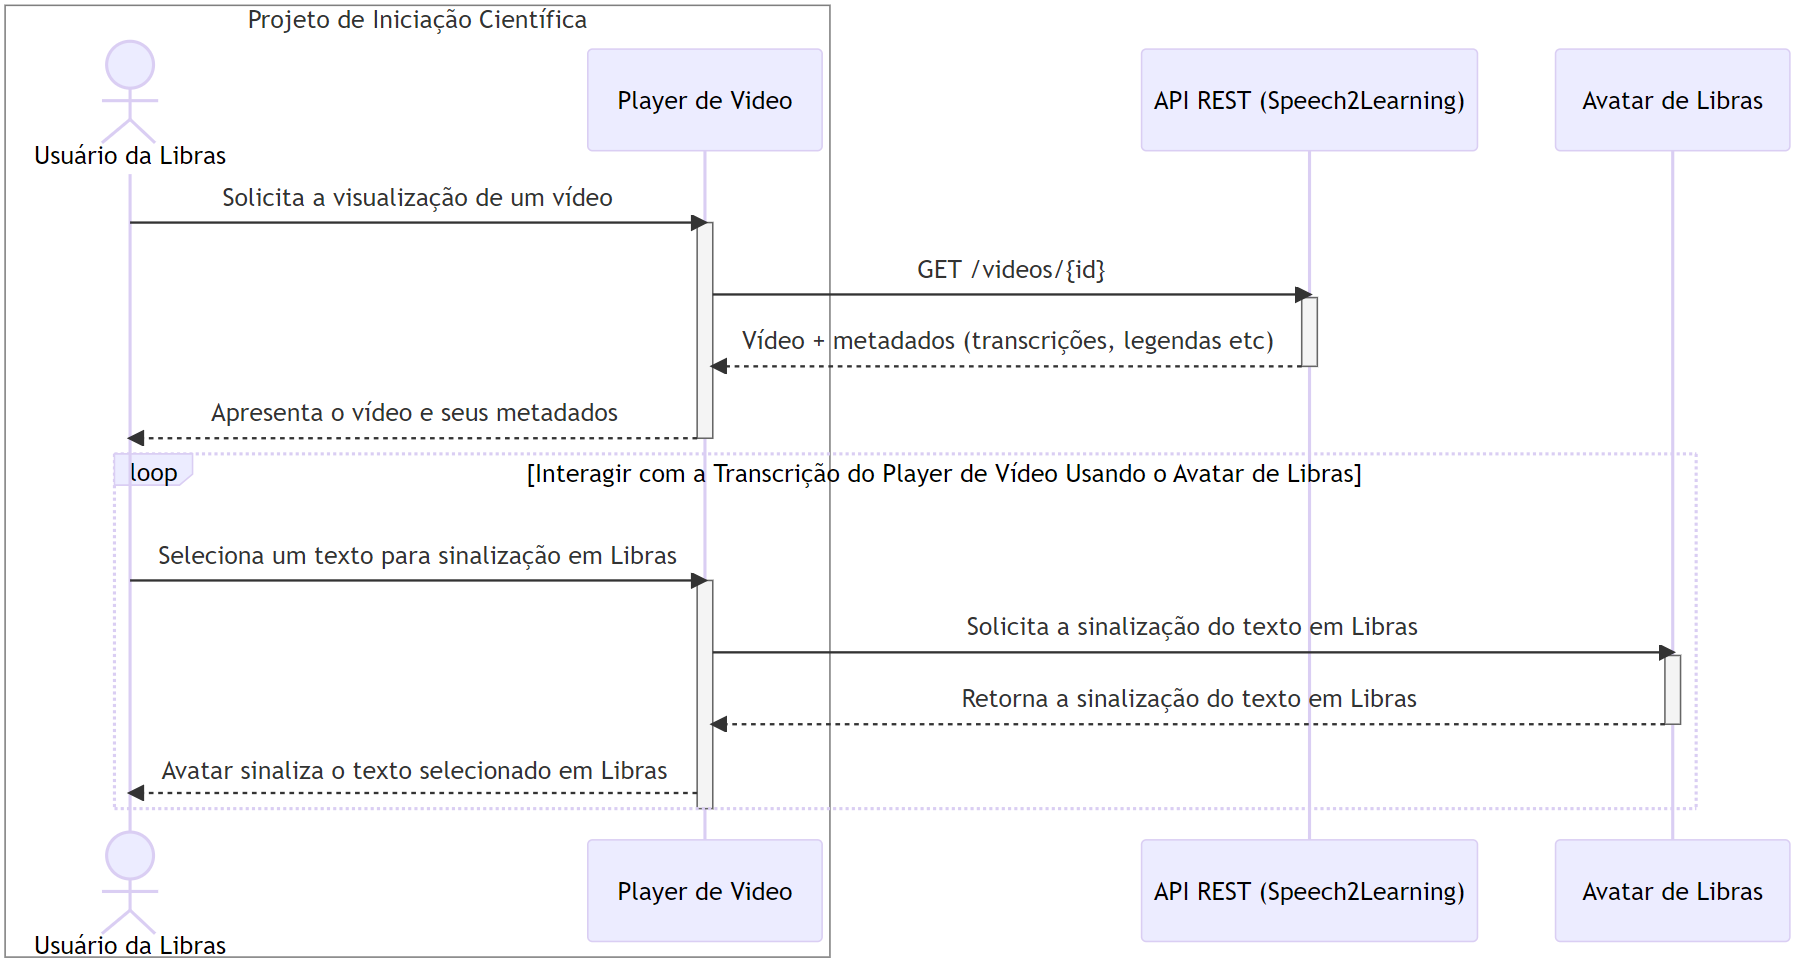
\includegraphics[width=1\textwidth]{images/chapter4-cs2-poc-diagram.png}
\fautor
\end{figure}

A integração entre o \textit{player} de vídeo e a API REST ilustra a capacidade da arquitetura \textit{Speech2Learning} de fomentar ambientes educacionais mais inclusivos. Adotando esta abordagem, os desenvolvedores podem criar sistemas robustos, tecnologicamente independentes e flexíveis, capazes de atender às especificidades de cada projeto.

O objetivo central deste estudo de caso é projetar, construir e avaliar um \textit{player} de vídeo que siga as recomendações do ``Guia de Boas Práticas para Acessibilidade Digital'' definidas por \citeonline{GovBr2023}, além dos princípios de \textit{Design} Universal promovidos pela \citeonline{UNESCO2023}. Este \textit{player}, integrado com a arquitetura \textit{Speech2Learning}, visa promover a educação inclusiva para surdos através da Libras.

Tecnicamente, o \textit{player} foi implementado utilizando HTML, CSS e JavaScript de forma ``pura'' (\textit{vanilla}), ou seja, evitando bibliotecas e/ou implementações alternativas para uma solução mais padronizada e manutenível baseada na Web \cite{GovBr2023}. Os \textit{wireframes} preliminares na Figura \ref{fig:chapter4-cs2-poc-wireframes} oferecem uma visão simplificada, destacando características universais e o símbolo ``Acessível em Libras'', sublinhando o compromisso com a educação inclusiva.

\begin{figure}[htbp]
\centering
\caption{\textit{Wireframes} do \textit{Player} de Vídeo Acessível (Modos Claro e Escuro)}
\label{fig:chapter4-cs2-poc-wireframes}
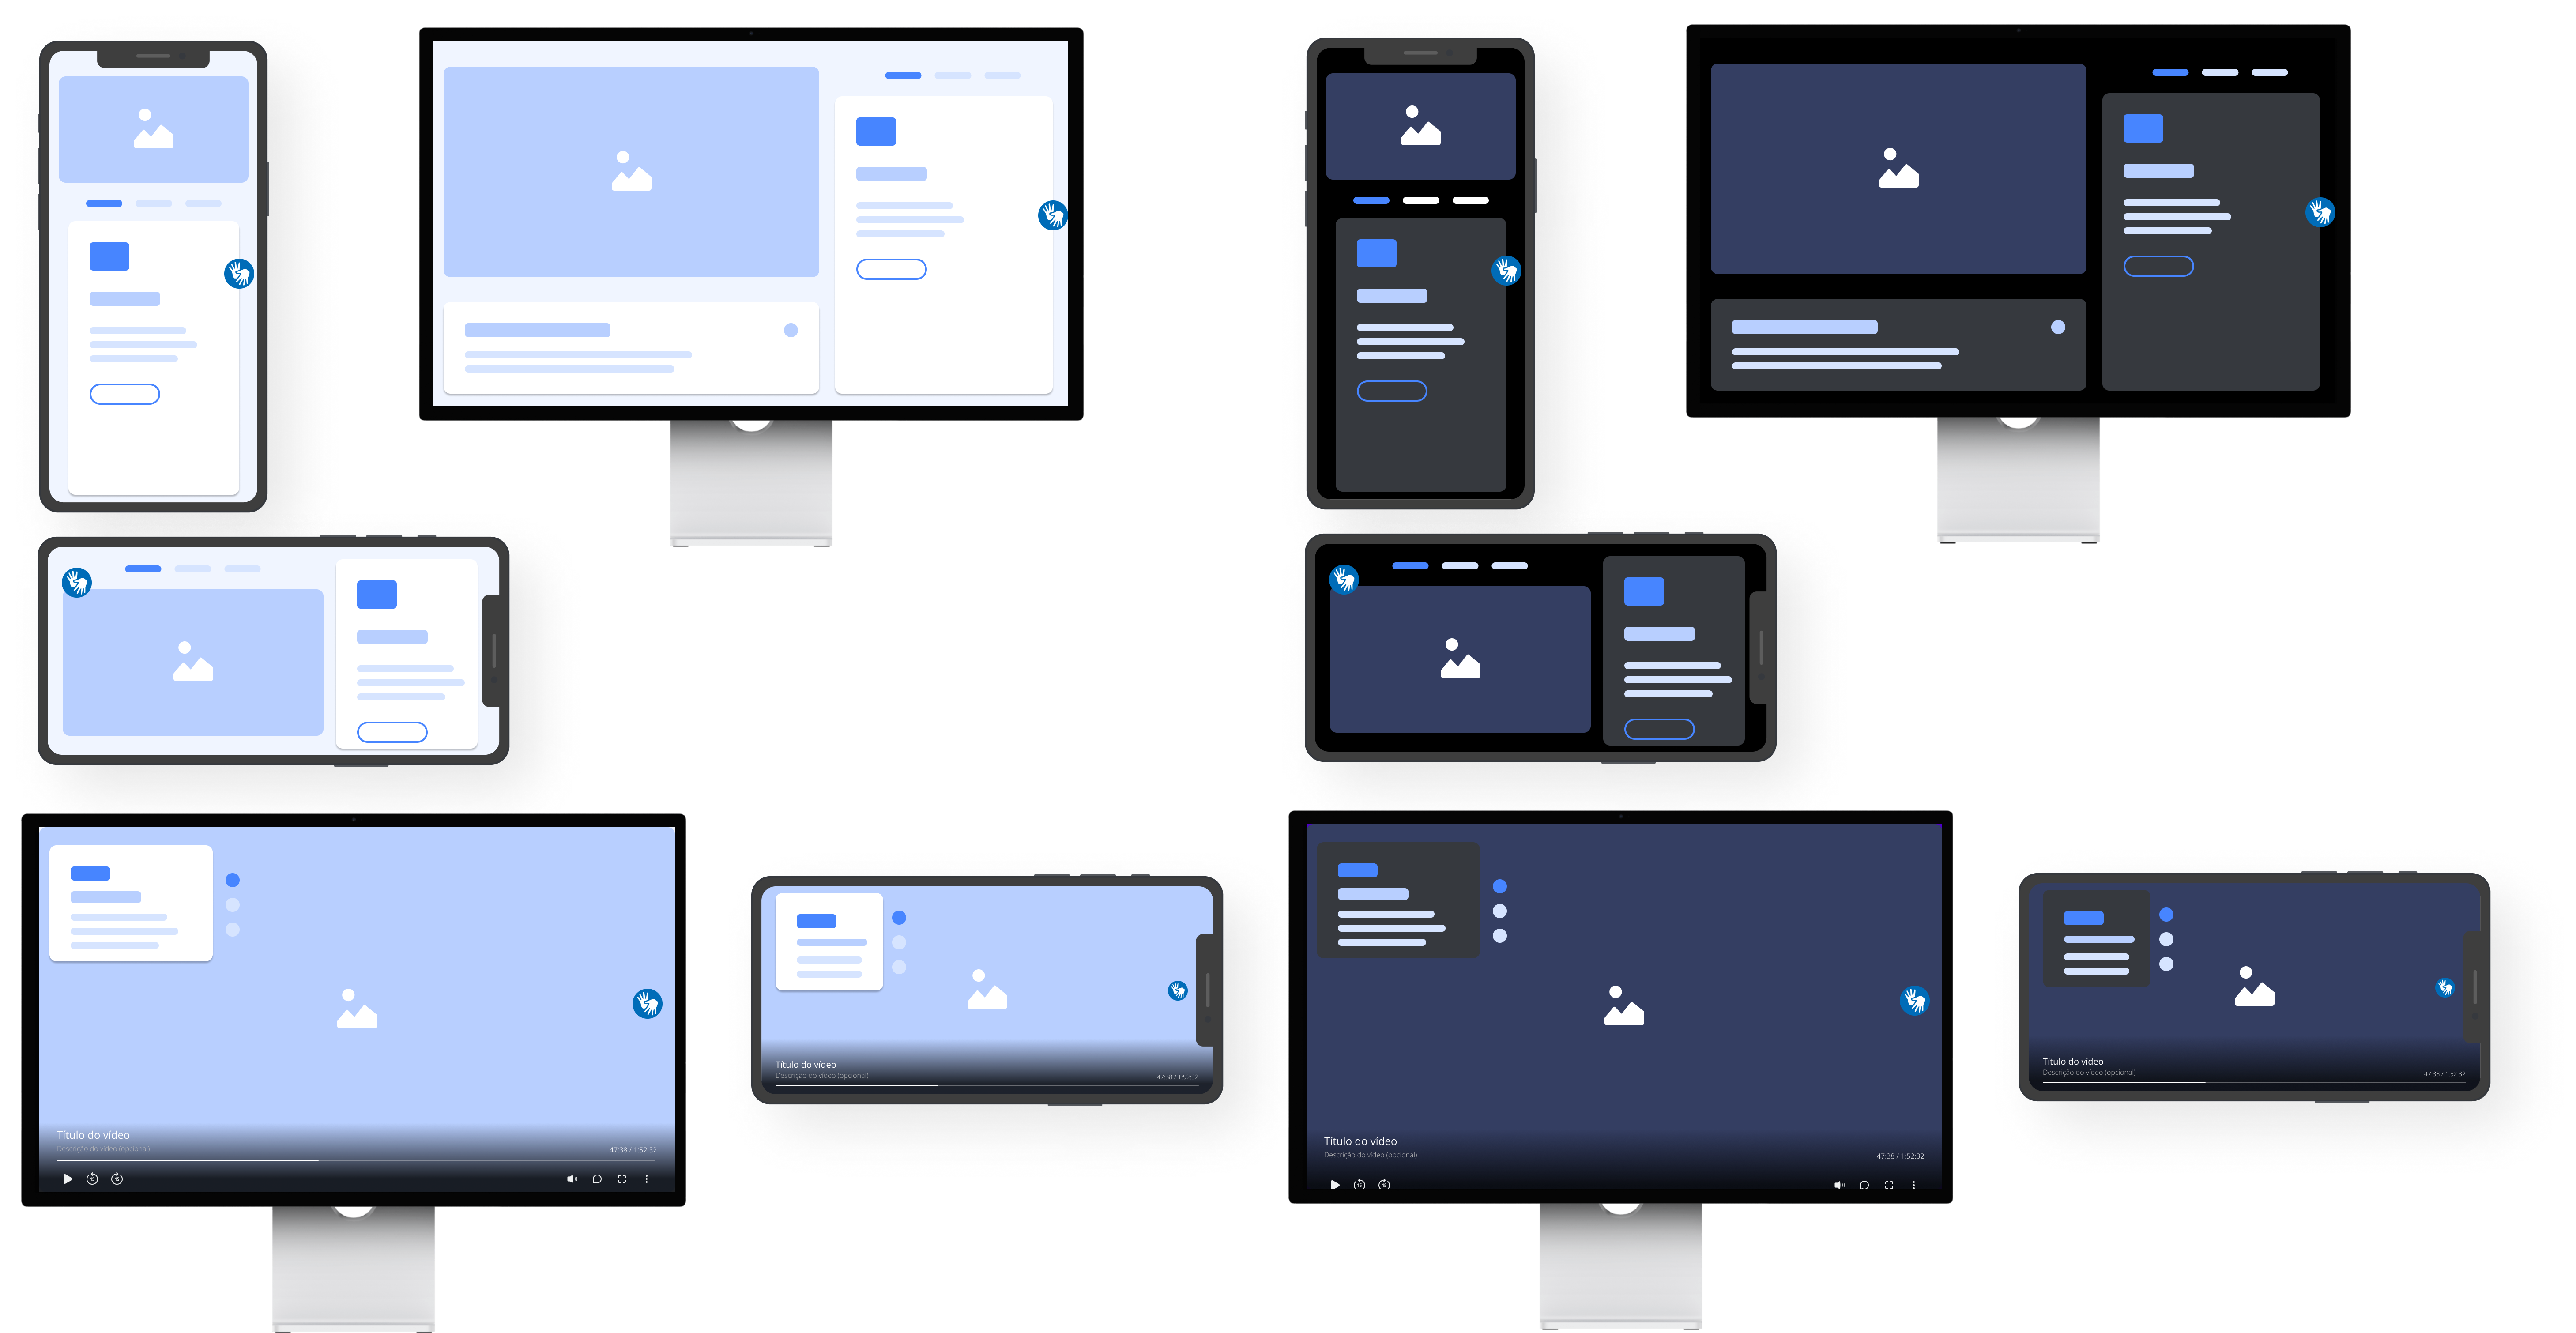
\includegraphics[width=1\textwidth]{images/chapter4-cs2-poc-wireframes.png}
\fautor
\end{figure}

Em particular, esta POC foi conduzida no contexto de dois projetos de \sigla{IC}{Iniciação Científica} vinculados a este doutorado, cada um explorando uma faceta essencial da solução proposta:

\begin{itemize}
\item \textbf{``\textit{Design} Acessível de um \textit{Player} de Vídeo com Transcrições em Libras: Uma Aplicação da Arquitetura \textit{Speech2Learning}''}: Projeto conduzido pela aluna Melissa Motoki Nogueira, com apoio do Programa Unificado de Bolsas (PUB) da USP. O objetivo foi aplicar os princípios do \textit{Design} Universal no desenvolvimento do \textit{player}, garantindo sua acessibilidade e inclusão para o maior número possível de usuários.

\item \textbf{``Estudo e Desenvolvimento de um \textit{Player} de Vídeo Acessível para Libras Explorando a Arquitetura \textit{Speech2Learning}''}: Projeto desenvolvido pelo aluno Adriano da Silva de Carvalho, com financiamento do PUB da USP. O foco foi construir o \textit{player} de vídeo como uma biblioteca aberta e flexível, facilitando sua integração em diversas plataformas e contextos educacionais, ampliando seu alcance e impacto.
\end{itemize}

\subsection{Metodologia}

Para investigar o impacto e a eficácia do \textit{player} de vídeo com avatares de Libras baseados em texto, adotou-se uma abordagem exploratória, visando gerar conhecimento sobre um fenômeno ainda pouco conhecido \cite{CastroFilho2021}. Este estudo de caso busca atingir dois objetivos principais: (i) investigar o impacto de avatares de Libras na acessibilidade de conteúdos para surdos; e (ii) explorar a eficácia desses avatares, integrados à transcrição automática de videoaulas, para a compreensão de OAs audíveis. \textcolor{red}{Esses objetivos foram guiados pela seguinte questão de pesquisa:}

\begin{citacao}
\textcolor{red}{\textbf{QP do Estudo de Caso 2}: Como as tecnologias de ASR podem ser adaptadas para atender às necessidades de acessibilidade de usuários da Libras? (\autoref{chapter1:research-questions})}
\end{citacao}

Adotou-se uma metodologia de análise mista, integrando dados quantitativos e qualitativos. Inicialmente, um \textit{survey} foi disponibilizado a todos os intérpretes profissionais da QS Inclusão (\url{https://qsinclusao.com.br}), com dois participantes respondendo efetivamente, incluindo o diretor fundador da empresa, cuja participação acrescentou uma visão estratégica e gerencial ao estudo. No \textit{survey}, os intérpretes avaliaram quantitativamente as performances dos avatares \textit{VLibras} e \textit{Hand Talk}, baseados em transcrições automáticas de videoaulas. \textcolor{red}{Para guiar a análise quantitativa e explorar possíveis tendências, foram formuladas as seguintes hipóteses exploratórias, que poderão ser refinadas como hipóteses nulas e alternativas em estudos futuros com amostras maiores:}

\begin{itemize}
\item \textbf{H1}: Os avatares de Libras são úteis na compreensão de OAs audíveis transcritos automaticamente.
\item \textbf{H2}: Existe diferença na qualidade de sinalização entre os avatares \textit{VLibras} e \textit{Hand Talk} ao utilizar transcrições automáticas.
\end{itemize}

Complementando o \textit{survey}, cada intérprete teve a oportunidade de agendar uma entrevista, contribuindo com dados qualitativos que enriqueceram a análise. Essas entrevistas foram planejadas para explorar de modo mais aprofundado as percepções e experiências dos intérpretes com o uso do \textit{player} de vídeo e os avatares de Libras. A coleta de dados seguiu um protocolo semi-estruturado, garantindo que todas as áreas relevantes fossem abordadas.

A análise dos dados qualitativos foi realizada utilizando a TFD \cite{Charmaz2009}, uma metodologia que permite o desenvolvimento de teorias emergentes diretamente dos dados coletados. Este processo envolveu a codificação aberta, identificando e categorizando os principais temas nas respostas dos intérpretes de Libras. Com isso, foi possível assegurar que os temas emergissem naturalmente dos dados, proporcionando uma compreensão aprofundada das percepções e experiências dos participantes, sem preconceitos prévios.

Com o objetivo de ampliar a acessibilidade de conteúdos educacionais para alunos surdos, este estudo investigou a eficácia de um \textit{player} de vídeo acessível, integrado a avatares de Libras baseados em texto, como uma segunda instância da arquitetura \textit{Speech2Learning}. Especificamente, buscou-se:

\begin{itemize}
\item \textbf{Avaliar o impacto dos avatares de Libras na acessibilidade de OAs audíveis}, verificando se a combinação de transcrição automática e representação visual em Libras promove uma experiência de aprendizagem adequada.
\item \textbf{Analisar a viabilidade e a precisão dos avatares de Libras}, considerando-os como um complemento às estratégias de acessibilidade já existentes, alinhadas aos princípios do \textit{Design} Universal.
\item \textbf{Compreender as percepções dos intérpretes de Libras} sobre a usabilidade, a precisão e o impacto dos avatares integrados às transcrições automáticas, fornecendo \textit{insights} valiosos para o aprimoramento da solução.
\end{itemize}

O \autoref{quadro:c4:cs2-summary} resume a abordagem metodológica adotada, que inclui uma análise mista com dados qualitativos e quantitativos. Devido ao número de participantes, o foco dos resultados e discussões recai sobre os dados qualitativos das entrevistas com os intérpretes de Libras, complementados por \textit{feedbacks} formais obtidos em conferências científicas. A seguir, serão detalhadas as percepções dos intérpretes sobre o uso de avatares de Libras, fornecendo uma visão aprofundada dos desafios e benefícios identificados, essenciais para o desenvolvimento de práticas pedagógicas mais inclusivas e acessíveis.

\begin{quadro}[htb]
\centering
\caption{Síntese do Estudo de Caso 2: \textit{Player} de Vídeo com Avatar de Libras}
\label{quadro:c4:cs2-summary}
\begin{tabular}{C{3cm}|m{11.75cm}}\hline
\textbf{Objeto de Estudo} & \textit{Player} de vídeo com avatar de Libras baseado em texto, integrado à transcrições automáticas. \\\hline
\textbf{Perspectiva} & Exploratório \\\hline
\textbf{Característica} & Elaboração de conhecimentos ou levantamento de informação acerca do fenômeno ainda pouco conhecido \cite{CastroFilho2021}. \\\hline
\textbf{Objetivos} & \begin{tabular}[c]{@{}m{11.75cm}@{}}1. Investigar o impacto de avatares de Libras baseados em texto na acessibilidade de conteúdos para surdos. \\ 2. Explorar a eficácia de avatares de Libras integrados à transcrição automática de videoaulas para a compreensão de OAs audíveis.\end{tabular} \\\hline
\textbf{Questões de Pesquisa} & Como as tecnologias de ASR/STT podem ser adaptadas para atender às necessidades de acessibilidade de usuários da Libras? \\\hline
\textbf{Hipóteses} & \begin{tabular}[c]{@{}m{11.75cm}@{}}1. Os avatares de Libras são úteis na compreensão de OAs audíveis transcritos automaticamente. \\2. Existe diferença na qualidade de sinalização entre os avatares \textit{VLibras} e \textit{Hand Talk} ao utilizar transcrições automáticas.\end{tabular} \\\hline
\textbf{Fontes de Dados} & Dados quantitativos do \textit{survey} e dados qualitativos de entrevistas com intérpretes de Libras. \\\hline
\textbf{Método de Coleta de Dados} & \begin{tabular}[c]{@{}m{11.75cm}@{}}1. \textit{Survey}\\ 2. Entrevistas semi-estruturadas\end{tabular} \\\hline
\textbf{Tipo de Análise} & Mista (Quantitativa e Qualitativa) \\\hline
\end{tabular}
\end{quadro}

\subsection{Resultados e Discussões}

%Os estudos de caso desta tese foram aprovados pelo \sigla{CEP}{Comitê de Ética e Pesquisa}, sob o CAAE 78381524.3.0000.5390. Embora ambos os estudos tenham sido descritos no projeto submetido ao CEP, o foco principal recai sobre o Estudo de Caso 2, que inclui tanto análises quantitativas quanto qualitativas. O Estudo de Caso 1 se concentrou principalmente em análises quantitativas da precisão de transcrições automáticas, o que não exigiu submissão ética individual. Em contraste, o Estudo de Caso 2 envolveu um componente qualitativo mais robusto, justificado pela realização de entrevistas com intérpretes de Libras.

Para explorar o impacto dos avatares de Libras na acessibilidade de conteúdos educacionais, adotou-se uma abordagem mista. Como mencionado anteriormente, dois intérpretes de Libras da empresa QS Inclusão contribuíram para o estudo, respondendo ao \textit{survey} e participando das entrevistas subsequentes. O \textit{survey} foi projetado para capturar as percepções quantitativas dos intérpretes sobre a utilidade e a qualidade dos avatares \textit{VLibras} e \textit{Hand Talk}, com base em transcrições automáticas de videoaulas.

Os resultados detalhados do \textit{survey} podem ser acessados na planilha \url{https://bit.ly/S2L-CS2SurveyResp}, com a cópia do formulário disponível no \autoref{appendix:libras-survey} e também online em \url{https://bit.ly/S2L-CS2Survey}. A análise quantitativa desses dados contribuiu para uma exploração inicial das hipóteses de pesquisa, buscando indícios sobre a utilidade dos avatares na compreensão de OAs e possíveis diferenças na qualidade de sinalização entre os dois avatares.

Para complementar os dados quantitativos do \textit{survey}, os intérpretes foram convidados a participar de entrevistas semi-estruturadas. Essas entrevistas foram planejadas para aprofundar as percepções capturadas pelo \textit{survey}, permitindo uma análise qualitativa rica das experiências e opiniões dos intérpretes sobre o uso de avatares de Libras em conteúdos educacionais.

A análise dos dados, com base nos dois participantes revelou \textit{insights} relevantes sobre a precisão e a usabilidade dos avatares de Libras. Embora os resultados quantitativos sejam limitados, eles oferecem uma síntese da percepção dos intérpretes sobre a precisão dos avatares. Em contraste, os dados qualitativos, extraídos das entrevistas, proporcionam uma compreensão mais aprofundada das nuances e desafios associados à adoção dessas tecnologias.

Os dados quantitativos sugerem que tanto o \textit{VLibras} quanto o \textit{Hand Talk} apresentaram limitações significativas na sinalização, com ambos os avatares recebendo avaliações que destacam a presença de erros capazes de comprometer a compreensão completa dos OAs. Esses resultados, embora limitados em escopo, fornecem um plano de fundo importante para a análise dos dados qualitativos, que ofereceram \textit{insights} adicionais sobre os obstáculos e potencialidades no uso dessas ferramentas.

Por sua vez, a análise qualitativa foi conduzida com base na TFD e revelou temas centrais relacionados ao uso dos avatares de Libras. O roteiro completo das entrevistas com os intérpretes está disponível no \autoref{appendix:libras-interview}, assegurando transparência no processo de coleta de dados e permitindo a replicação dos métodos. Durante as entrevistas, o avatar \textit{VLibras} foi utilizado como a principal ferramenta de sinalização, priorizado em detrimento ao \textit{Hand Talk} devido a fatores como sua gratuidade, natureza \textit{open-source} e o suporte contínuo do governo brasileiro. %Além disso, o \textit{VLibras} oferece configurações avançadas de regionalidade e tem recebido atualizações frequentes nos últimos anos, tornando-o uma escolha adequada para este estudo.

%Embora os resultados das entrevistas ainda estejam sendo conduzidas, a integração dos dados qualitativos e quantitativos fornecerá uma visão mais abrangente e detalhada dos impactos e desafios na adoção dessas tecnologias. O roteiro completo para as entrevistas com os intérpretes está disponível no \autoref{appendix:libras-interview}, assegurando transparência no processo de coleta de dados e permitindo a reprodutibilidade dos métodos.

%Na prática, tendo em vista o nosso planejamento e previsão financeira, utilizamos apenas o \textit{VLibras} como avatar de Libras. Ele foi priorizado em detrimento ao \textit{Hand Talk} por ser gratuito, \textit{open-source} e mantido pelo governo brasileiro. Além disso, possui configurações avançadas relacionadas à regionalidade e, nos últimos anos, voltou a ser atualizado com frequência.

As entrevistas foram transcritas e submetidas a um processo de codificação aberta, axial e seletiva \cite{Charmaz2009}. Durante a codificação aberta, segmentos de texto foram categorizados em conceitos iniciais. Em seguida, na codificação axial, esses conceitos foram organizados em categorias mais amplas, que estabelecem relações entre os diferentes conceitos identificados. Finalmente, a codificação seletiva sintetizou essas categorias em um tema central que reflete a percepção geral dos intérpretes sobre o \textit{player} de vídeo.

Os intérpretes de Libras reconheceram que as transcrições automáticas utilizadas pelo \textit{player} de vídeo apresentaram um alto nível de precisão, um fator já validado no primeiro estudo de caso desta pesquisa. No entanto, a integração dessas transcrições com avatares de Libras revelou desafios significativos. A principal dificuldade mencionada pelos intérpretes está na incapacidade dos avatares de incluir o contexto apropriado em suas sinalizações, o que pode comprometer a transferência de conhecimento. A Libras, como uma língua visual-espacial, depende fortemente do contexto para a correta interpretação dos sinais \cite{Quadros2017, Quadros2019, Honora2021}. Quando este contexto não é adequadamente sinalizado pelo avatar, a mensagem pode se tornar incoerente ou incompleta, prejudicando o entendimento do conteúdo.

Outro ponto levantado pelos intérpretes refere-se às barreiras sociais enfrentadas por muitos surdos e pessoas com deficiência auditiva. Grande parte dessa população não tem a oportunidade de ser bilíngue (fluente em Libras e Português) ou oralizada, o que significa que essas pessoas dependem exclusivamente da Libras para acessar o conteúdo educacional. Quando o avatar falha em proporcionar uma sinalização coerente, esses usuários ficam em desvantagem, pois não têm outra forma de acessar a informação. Essa questão ressalta a importância de desenvolver soluções tecnológicas que não só sejam tecnicamente avançadas, mas também culturalmente sensíveis e inclusivas.

Por outro lado, os intérpretes também destacaram o potencial das novas tecnologias de IA para transformar o campo da acessibilidade. Modelos de IA estão sendo treinados especificamente em Libras, o que promete inaugurar uma nova era de acessibilidade para a comunidade surda. Um exemplo citado nas entrevistas foi a iniciativa da Lenovo, que desenvolveu uma solução de tradução em tempo real para a Libras impulsionada por IA, mostrando resultados promissores \cite{Lenovo2023}. Esses avanços tecnológicos são vistos como oportunidades para superar as limitações atuais dos avatares de Libras e oferecer soluções mais eficazes e inclusivas no futuro.

A análise das entrevistas indica que, embora o \textit{player} de vídeo desenvolvido como uma instância da arquitetura \textit{Speech2Learning} seja um passo significativo, há áreas críticas que precisam de melhorias. A principal delas é a integração de avatares de Libras que possam incluir o contexto necessário para uma comunicação assertiva. Além disso, as barreiras sociais e linguísticas enfrentadas por muitos surdos devem ser levadas em consideração no desenvolvimento de futuras soluções. O surgimento de soluções baseadas em IA, como os modelos mencionados pelos intérpretes, deve ser explorada para criar soluções que ofereçam uma tradução mais precisa e culturalmente adequada. O \autoref{quadro:c4:cs2-grounded-theory} sumariza as categorias e temas identificados na análise das entrevistas, utilizando a técnica da TFD.

\begin{quadro}[htb]
\centering
\caption{Categorias e Temas Identificados na Análise das Entrevistas}
\label{quadro:c4:cs2-grounded-theory}
\begin{tabular}{l|p{10cm}}
\hline
\textbf{Categoria/Tema}              & \textbf{Descrição}                                                                 \\ \hline
\textbf{Acessibilidade}         & Avaliação sobre como o \textit{player} facilita o acesso à informação para usuários surdos.  \\ \hline
\textbf{Qualidade Linguística}  & Percepção sobre a exatidão e clareza das transcrições automáticas.                 \\ \hline
\textbf{Experiência do Usuário} & Comentários sobre a interface e facilidade de uso do \textit{player}.                                \\ \hline
\textbf{Integração com Avatares}& Reflexões sobre a compatibilidade cultural e linguística dos avatares de Libras.    \\ \hline
\textbf{Desafios e Limitações}  & Dificuldades técnicas e limitações enfrentadas durante o uso do \textit{player}.            \\ \hline
\textbf{Barreiras Sociais}      & Discussões sobre as barreiras enfrentadas por surdos não bilíngues ou não oralizados.\\ \hline
\textbf{Oportunidades com IA}   & Potencial dos novos modelos de IA especializados em Libras para melhorar a acessibilidade e a inclusão de surdos.                  \\ \hline
\end{tabular}
\end{quadro}

De forma complementar, é importante destacar que o \textit{player} foi apresentado no \textit{``Workshop on Opportunities and Challenges of Generative AI in Education''}, parte da \textit{``57th Hawaii International Conference on System Sciences (HICSS)''}, onde a arquitetura \textit{Speech2Learning} foi formalmente publicada em um paper completo \cite{FalvoJr2023_HICSS}. A \autoref{fig:chapter4-cs2-poc-demo} mostra as etapas da demonstração: (a) \textit{Player} de vídeo integrado às transcrições automáticas em múltiplos idiomas; (b) Avatar \textit{VLibras} ativado e sinalizando um paragrafo da transcrição; e (c) Configurações de regionalismo disponíveis no \textit{VLibras}. Seguem algumas dúvidas e \textit{feedbacks} relevantes deste evento:

\begin{figure}[htbp]
\centering
\caption{\textit{Screenshots} da Demo do \textit{Player} de Vídeo.}
\label{fig:chapter4-cs2-poc-demo}
\begin{subfigure}[b]{0.83\textwidth}
\centering
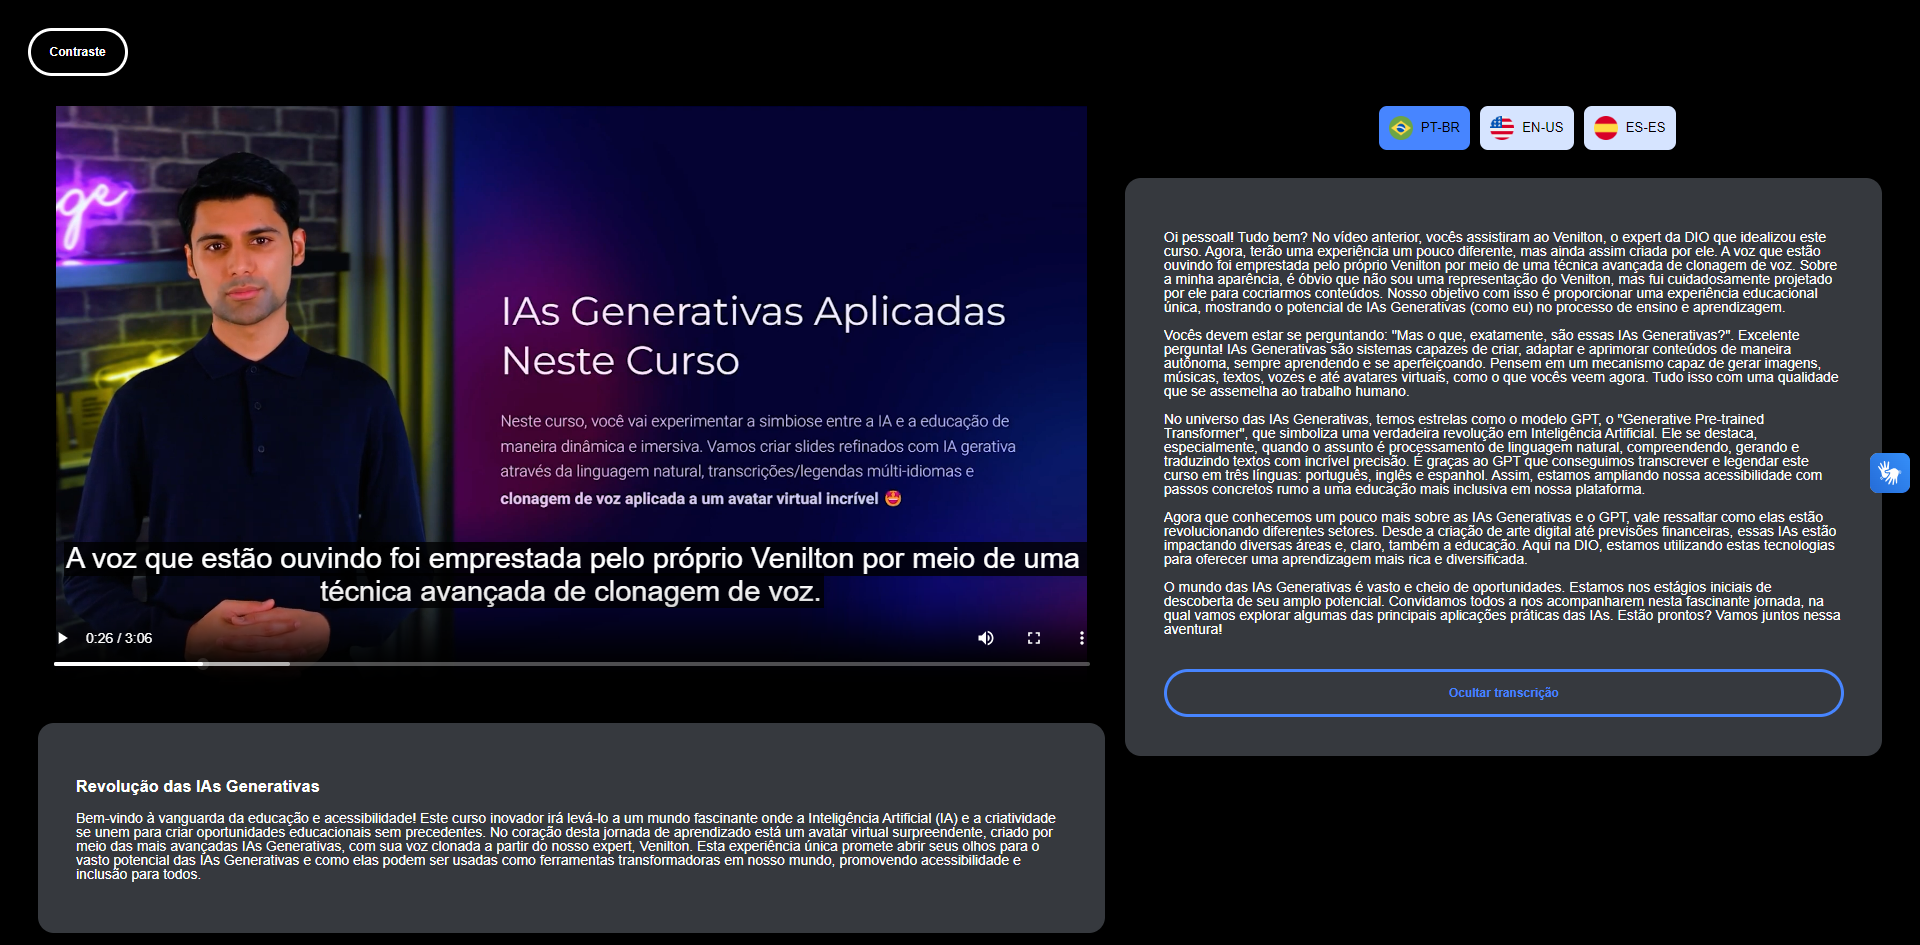
\includegraphics[width=\textwidth]{images/chapter4-cs2-poc-demo1.png}
\caption{\textit{Player} de Vídeo: Transcrições e Legendas.}
\label{fig:chapter4-cs2-poc-demo1}
\end{subfigure} ~
\begin{subfigure}[b]{0.83\textwidth}
\centering
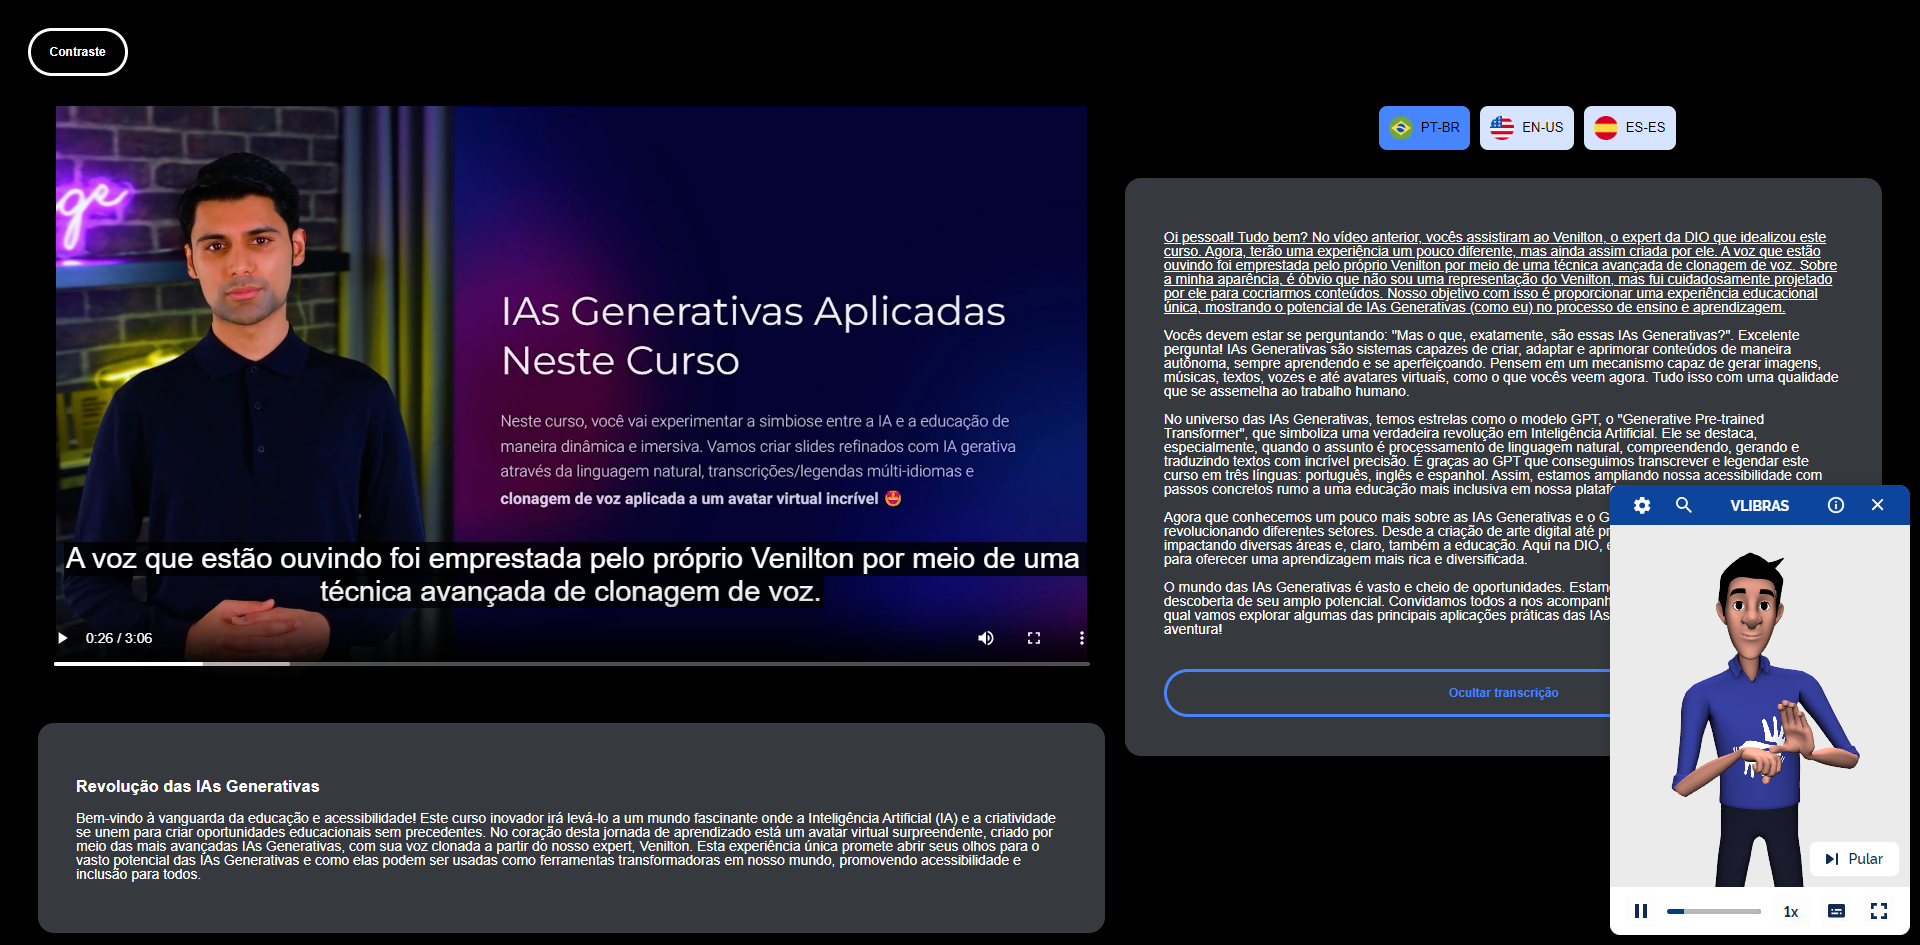
\includegraphics[width=\textwidth]{images/chapter4-cs2-poc-demo2.png}
\caption{\textit{Player} de Vídeo: Avatar de Libras (VLibras) Sinalizando.}
\label{fig:chapter4-cs2-poc-demo2}
\end{subfigure} ~
\begin{subfigure}[b]{0.83\textwidth}
\centering
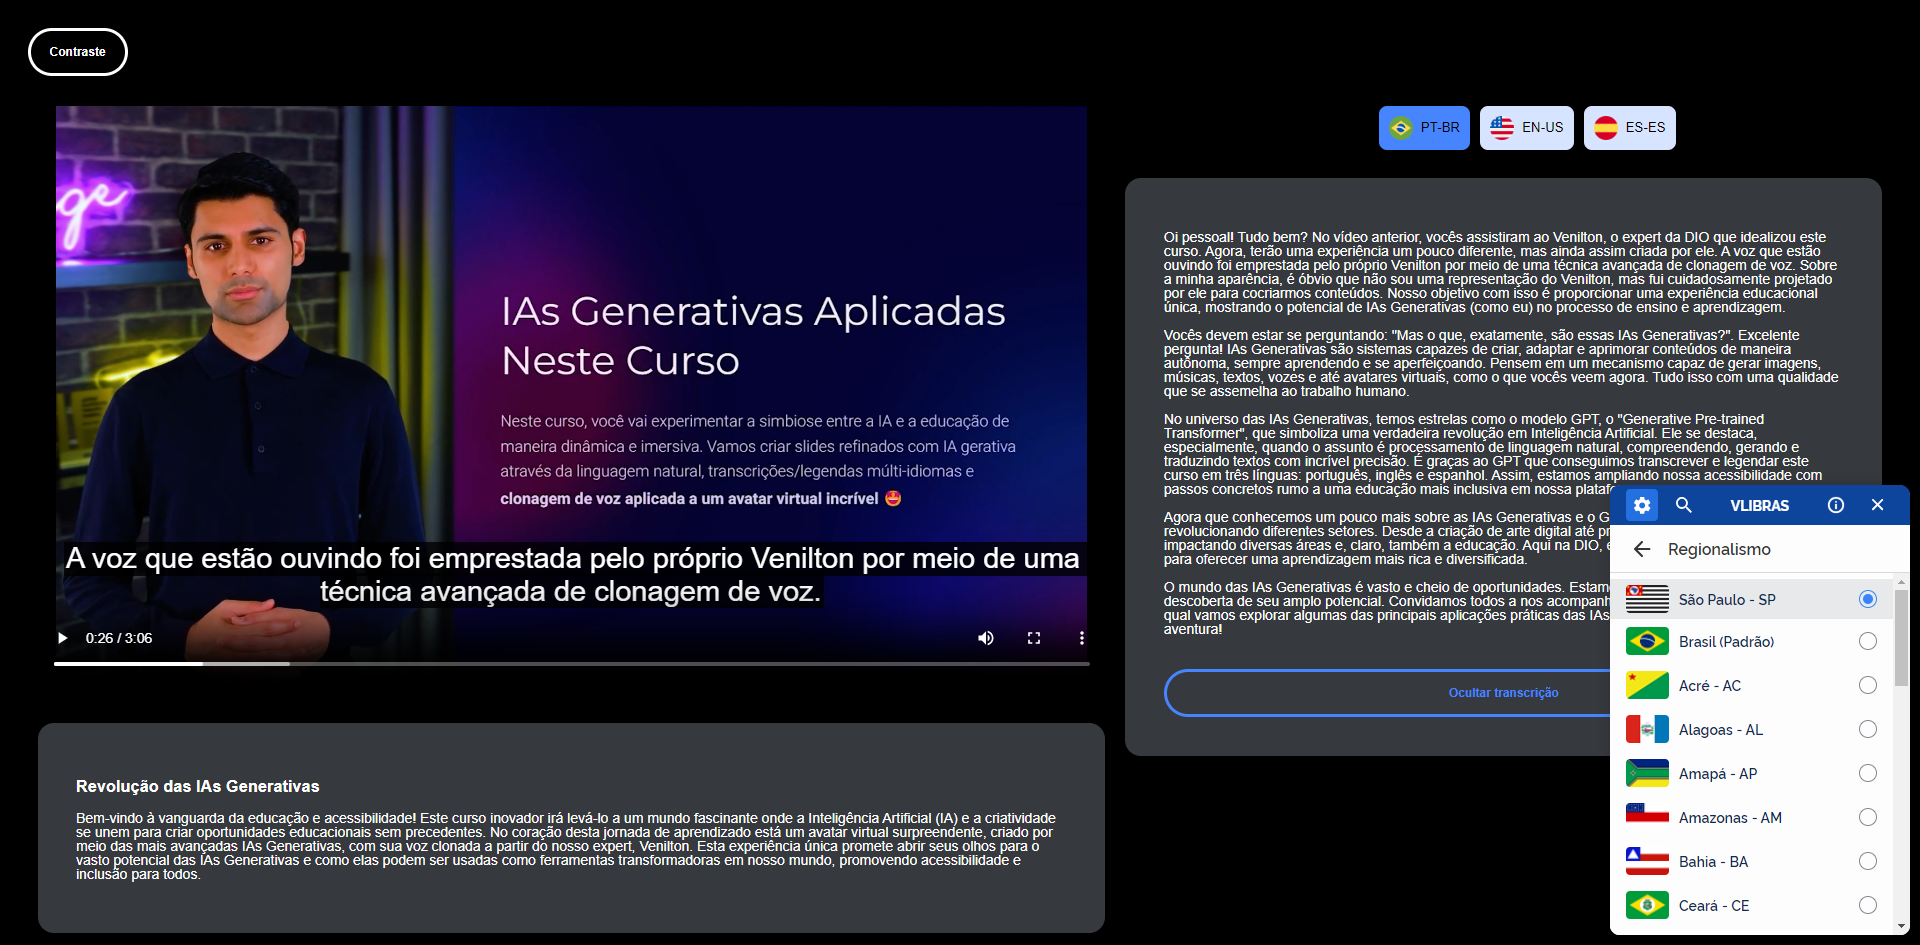
\includegraphics[width=\textwidth]{images/chapter4-cs2-poc-demo3.png}
\caption{\textit{Player} de Vídeo: Avatar de Libras (VLibras) Regionalismo.}
\label{fig:chapter4-cs2-poc-demo3}
\end{subfigure}
\fautor
\end{figure}

\begin{itemize}
    \item \textbf{Como lidar com as variações regionais das próprias línguas de sinais?}
    
    É fundamental reconhecer a importância das regionalidades e sotaques tanto na língua falada quanto na sinalizada. A variação regional é uma característica intrínseca das línguas de sinais, que varia conforme a localização geográfica. No estudo, o \textit{VLibras}, que possui configurações de regionalidade para cada estado do Brasil, foi utilizado para que o avatar considerasse essas variações ao sinalizar. Este aspecto é crucial para a aceitação e eficácia do avatar de Libras, pois respeita as particularidades culturais e linguísticas dos usuários.
    \item \textbf{Qual seria o esforço para integrar o \textit{player} de vídeo a avatares de outras línguas de sinais, como a ASL?}
    
    O \textit{player} foi implementado seguindo as práticas de \textit{Design} Universal, que preconizam que as soluções atendam ao maior número possível de usuários. O \textit{player} é, essencialmente, uma biblioteca HTML, CSS e JavaScript, garantindo que o \textit{player} de vídeo HTML, bem como sua descrição, transcrições e legendas, sigam as boas práticas de semântica, estilos e interações. Dessa forma, o \textit{player} não precisa ``conhecer'' o avatar de língua de sinais específico, pois está preparado estruturalmente para integrá-lo, facilitando a adaptação para outras línguas de sinais, como a ASL.
    \item \textbf{Como as IAGen estão ajudando no desenvolvimento de projetos relacionados à Arquitetura \textit{Speech2Learning}?}
    
    Os modelos de ML têm evoluído consideravelmente nos últimos anos, e atualmente é comum ouvir sobre GPT e outras siglas relacionadas à IA. As tecnologias de ASR e STT têm se beneficiado amplamente dessa revolução. O modelo de reconhecimento de fala da OpenAI, chamado Whisper, é baseado na tecnologia \textit{Transformers}, a mesma utilizada no ChatGPT. Notavelmente, o Whisper se destacou nos testes e análises estatísticas, sendo escolhido como provedor padrão para a API de transcrição e legendagem de videoaulas devido à sua precisão e confiabilidade.
\end{itemize}

O estudo de caso realizado sobre o \textit{player} de vídeo com Avatar de Libras ilustra o progresso feito na inclusão educacional para alunos surdos. A implementação da arquitetura \textit{Speech2Learning} e a utilização dos avatares de Libras, como o \textit{VLibras}, têm demonstrado avanços na acessibilidade de conteúdos educacionais, respeitando as particularidades regionais e culturais dos usuários. %Os \textit{feedbacks} recebidos no HICSS reforçam a relevância e a aplicabilidade da solução proposta, sublinhando a importância de continuar explorando e aperfeiçoando tecnologias assistivas no contexto educacional.

A abordagem mista adotada para investigar a eficácia dos avatares de Libras envolveu a aplicação de um \textit{survey} e a realização de entrevistas com intérpretes de Libras. A partir dos dados obtidos, as hipóteses formuladas foram: (i) Os avatares de Libras são úteis na compreensão de OAs audíveis transcritos automaticamente; e (ii) Existe uma diferença na qualidade de sinalização entre os avatares \textit{VLibras} e \textit{Hand Talk} ao utilizar transcrições automáticas.

No entanto, a análise dos resultados não fornece uma confirmação conclusiva dessas hipóteses. O \textit{survey} revelou percepções valiosas sobre a utilidade e a qualidade dos avatares, mas a amostra limitada de participantes e a diversidade das respostas obtidas indicam que mais pesquisas são necessárias para validar e generalizar esses achados. A questão de pesquisa, que explora como as tecnologias de reconhecimento de fala (ASR/STT) podem contribuir para uma educação mais acessível para usuários da Libras, continua sendo relevante, mas os dados atuais sugerem que os resultados devem ser interpretados com cautela.

Para concluir, a \textit{Speech2Learning} oferece um arcabouço genérico e aberto às tendências emergentes das IAs, possibilitando uma evolução natural em suas soluções de TA derivadas. Contudo, é fundamental prosseguir com estudos adicionais para refinar e avaliar sua eficácia em contextos variados. A continuidade da pesquisa permitirá aprimorar a precisão dos avatares e a integração de novas abordagens que potencializem ainda mais a acessibilidade educacional.

\section{Considerações Finais}

Os dois estudos de caso apresentados neste capítulo ressaltam a importância e a viabilidade de utilizar tecnologias de reconhecimento de fala para promover ambientes de ensino-aprendizagem mais acessíveis, destacando o papel central da arquitetura \textit{Speech2Learning} como diretriz no desenvolvimento de recursos de TA. 

No primeiro estudo de caso, focado em legendas automáticas para videoaulas, observou-se que transcrições automáticas precisas podem aumentar significativamente o potencial de reuso e acessibilidade de OAs audíveis, alinhando-se com uma das premissas fundamentais da arquitetura proposta. As contribuições deste estudo foram discutidas em publicações recentes, destacando a idealização da \textit{Speech2Learning}, a análise léxica das transcrições automáticas e a triangulação de dados para avaliar a acessibilidade dos OAs audíveis:

\begin{itemize}
    \item \citeonline{FalvoJr2023_HICSS}: \fullcite{FALVOJR, V.; MARCOLINO, A.; BRUNO, D.; MARTINS FALVO, C.; OSÓRIO, F.; BARBOSA, E.}{Lexical Analysis of Automatic Transcriptions Using Speech-to-Text Services: A Statistically Evaluated Case Study}{Hawaii International Conference on System Sciences (HICSS)}{2024}{Disponível em \url{hdl.handle.net/10125/107023}}

    \item \citeonline{FalvoJr2024_FIE}: \fullcite{FALVOJR, V.; MARCOLINO, A.; BRUNO, D.; MARTINS FALVO, C.; OSÓRIO, F.; BARBOSA, E.}{Enhancing Learning Objects Accessibility Through Speech-To-Text Based Architecture: A Comprehensive Triangulation Study}{Frontiers in Education (FIE)}{2024}{Submetido em 20/05/2024 e aceito em 23/07/2024}
\end{itemize}

O segundo estudo de caso envolveu o desenvolvimento de um \textit{player} de vídeo com \textit{Design} Universal, integrando transcrições automáticas e avatares de Libras baseados em texto. Esse estudo reforçou o potencial da arquitetura \textit{Speech2Learning} em atender algumas das necessidades da comunidade surda, mas também revelou limitações significativas. Esses desafios sublinham a importância de futuras iterações da arquitetura, visando otimizar sua aplicabilidade em diferentes contextos e grupos de usuários, promovendo um processo de ensino-aprendizagem mais inclusivo.

Os resultados obtidos até o momento indicam que a integração de tecnologias como ASR/STT com soluções educacionais pode facilitar uma educação mais inclusiva e acessível. A continuidade deste trabalho incluirá a análise detalhada dos dados coletados nas entrevistas com intérpretes de Libras. Além disso, pesquisas futuras podem explorar a adaptação de avatares de outras línguas de sinais e o uso de novas tecnologias de IA para aprimorar ainda mais as soluções desenvolvidas com base na arquitetura proposta.

Em síntese, os estudos de caso apresentados neste capítulo representam um avanço significativo na direção de uma educação verdadeiramente inclusiva. A aplicação da arquitetura \textit{Speech2Learning} e o uso de avatares de Libras destacam-se como abordagens promissoras para promover a inclusão educacional, contribuindo para a construção de um ambiente educacional mais acessível.

No próximo capítulo serão discutidas as principais contribuições e limitações desta pesquisa, além de propostas para trabalhos futuros. Também será apresentada uma lista completa das publicações resultantes deste trabalho, consolidando os avanços alcançados e apontando caminhos para o desenvolvimento contínuo no campo da acessibilidade educacional.
